\documentclass[twoside, final, 11pt]{articleMine}
\usepackage[english]{babel} \usepackage{a4wide}
\usepackage{amsmath,amssymb,accents} \usepackage{epsfig}
\usepackage{subfigure} \usepackage{units} \usepackage{graphicx}
\usepackage[displaymath, mathlines, right]{lineno} \usepackage{xspace}
\usepackage{color} \usepackage{epic,eepic,pstricks}
\usepackage{acronym} \usepackage{wrapfig,multicol}
\usepackage{deluxetable} \usepackage{todonotes} 
\usepackage{hyperref}
\usepackage{float}
%\usepackage{slashbox}
\usepackage{lmodern} 
%\usepackage{caption}
\linenumbers
%\usepackage{showlabels}
\usepackage[draft]{showkeys}

%\usepackage[nolists, tablesfirst]{endfloat}
\graphicspath{{plots/}}
\newcommand*\patchAmsMathEnvironmentForLineno[1]{%
  \expandafter\let\csname old#1\expandafter\endcsname\csname #1\endcsname
  \expandafter\let\csname oldend#1\expandafter\endcsname\csname end#1\endcsname
  \renewenvironment{#1}%
     {\linenomath\csname old#1\endcsname}%
     {\csname oldend#1\endcsname\endlinenomath}}%
\newcommand*\patchBothAmsMathEnvironmentsForLineno[1]{%
  \patchAmsMathEnvironmentForLineno{#1}%
  \patchAmsMathEnvironmentForLineno{#1*}}%
\AtBeginDocument{%
\patchBothAmsMathEnvironmentsForLineno{equation}%
\patchBothAmsMathEnvironmentsForLineno{align}%
\patchBothAmsMathEnvironmentsForLineno{flalign}%
\patchBothAmsMathEnvironmentsForLineno{alignat}%
\patchBothAmsMathEnvironmentsForLineno{gather}%
\patchBothAmsMathEnvironmentsForLineno{multline}%
}
%\AtBeginFigures{\cleardoublepage}
%%%%%\parindent 5pt  
\parskip 1.2pt           % sets spacing between paragraphs
\def\Offline{\mbox{$\overline{\rm
Off}$\hspace{.05em}\raisebox{.4ex}{$\underline{\rm line}$}}\xspace}
\def\OfflineB{\mbox{$\bf\overline{\rm\bf
Off}$\hspace{.05em}\raisebox{.4ex}{$\bf\underline{\rm\bf line}$}}\xspace}

\def\eq#1{\begin{equation}#1\end{equation}}
%\def\al#1{\begin{align}#1\end{align}}
%\def\vc#1{{\bf #1}}
\def\pt#1{\accentset{\rightharpoonup}{#1}}
\include{myabbr}

\newcommand{\HRule}{\rule{\linewidth}{0.5mm}}
\newcommand{\VEM}{\mbox{VEM}}
\newcommand{\m}{\mbox{m}}

\let\stdsection\section  
%\renewcommand\section{\newpage\stdsection}  
 
\begin{document}

%\setpagewiselinenumbers
\modulolinenumbers[2]

%\linenumbers


\renewcommand\linenumberfont{\small\rmfamily}
\begin{center}
  \vspace*{-13ex}

  \rule{\linewidth}{0.1mm}  \\[17mm] {\huge  Installation of the new electronics for the Helix array (Malargue December 2016)}
     \begin{flushright}
       \small 
     
     \end{flushright}

  % 
\end{center}
% 
\vspace*{2ex} 
%
\thispagestyle{empty}
\noindent
\begin{abstract}
  \noindent
  We  present here a  first report  on the  installation of  the helix
  antennas   with  the   new   electronics.   We   show  also   onsite
  measurements.
\end{abstract}
\begin{figure}[ht!]
  \centering
  \hspace*{-3ex}
%%  \subfigure{\includegraphics[width=0.49\linewidth]{/Users/romain/work/Auger/EASIER/LPNHE/notes/tex/installhelix/plotsantoinehelix.jpg}}
  \subfigure{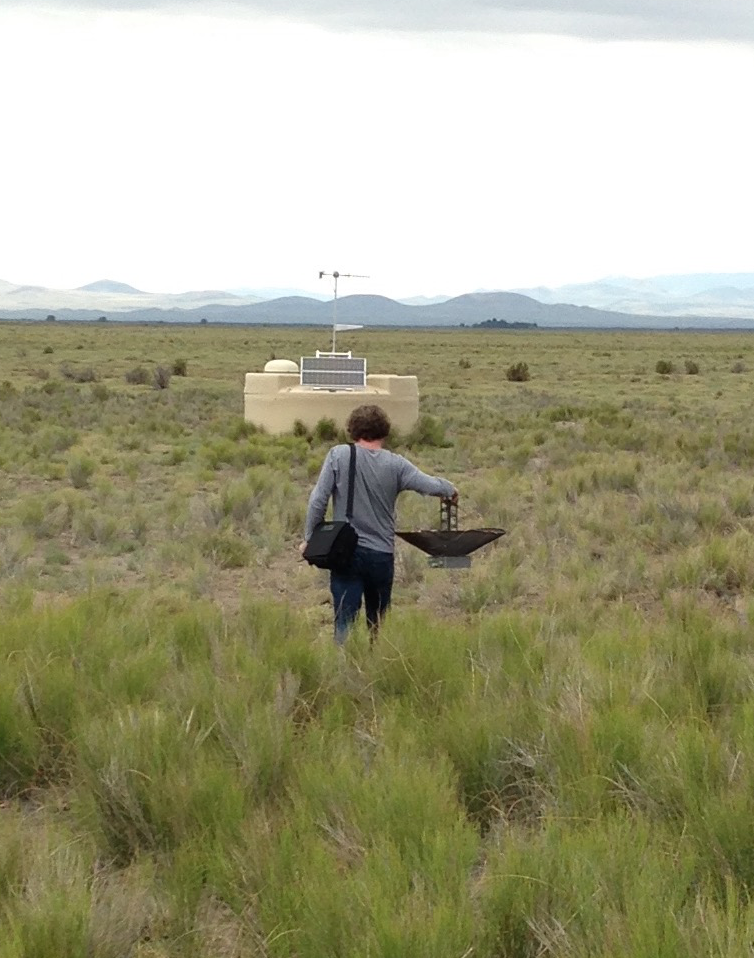
\includegraphics[width=0.49\linewidth]{antoinehelix.png}}
  \label{fig:monit}
\end{figure}
%
\thispagestyle{empty}
%$\;$
%\listoftodos
%\newpage
\noindent
\section{Introduction}
The setup in the L-band (1-1.5GHz)  was installed in march 2015. It is
composed of  an helix antenna,  an amplifier stage, and  an adaptation
stage. The  data collected in  2015 showed no sensitivity  and strange
behavior. In  May 2016 all the  detectors from the  helix hexagon were
removed  and  tested~\cite{helixstatusmay2016}.  Several  issues  were
spotted:
\begin{itemize}
\item mechanical: the ring of the reflector was broken
\item  at  the amplifier  stage:  almost  all  the amplifiers  failed,
  probably due to electrostatic discharge (ESD).
\item the adaptation board had setting issues on the dynamic range
\end{itemize}
These issues  were addressed  by: reinforcing
the reflector's  ring and  putting ropes to  tie the reflector  to the
central part;  designing an amplifier  board with a ESD  protection at
its  entry   stage(description  and   calibration  can  be   found  in~\cite{lnatesting});  changing  a  few  components  on  the  adaptation
board.\\ We present here the  installation of the new setup with these
new features.

\section{Installation sum up}
The  antennas were  already  prepared,  we had  repaired  them in  May
2016. The electronics boxes were  brought from Paris for this trip. We
prepared 16 amplifier boxes (8 with  an input filter, 8 without) and 7
adaptation board boxes.
\subsection{preliminary tests}
Before performing the installation, we have two questions to answer:
\begin{itemize}
\item is the input filter necessary ?
\item    is    the    electric    line    located    on    the    road
  (see~Figure\ref{fig:hexagon}) a source of noise ?
\end{itemize}
The first day we went for a survey of the helix hexagon to be sure all
the tanks were easy to access. We also made measurements to answer the
questions  listed  above.    Figure~\ref{fig:filter}  (left)  shows  a
spectrum recorded  on the road close  to the tank Santy,  one is taken
without filter (blue) and the other with (green). The spectrum without
filter  shows a  ringing  behavior with  peaks  at regular  intervals.
These intervals are $\rm \simeq  100MHz$ long, so the ringing could be
caused by the  FM band.  Even if the spectrum in  our band of interest
seem  unchanged with  or  without  filter, we  cannot  operate with  a
saturated amplifier. We  choose the filtered version, even  if we know
the noise temperature is higher.
\begin{figure}[ht!]
  \centering
  \hspace*{-3ex}
  \subfigure{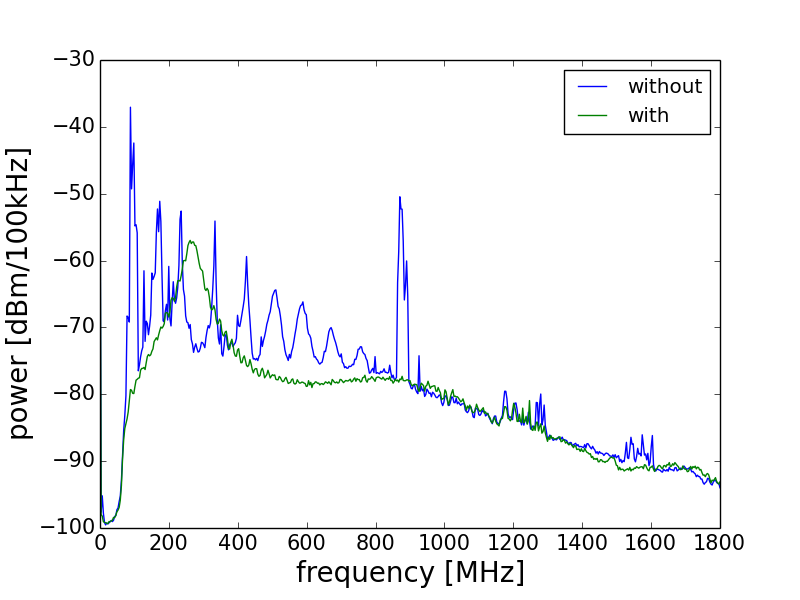
\includegraphics[width=0.49\linewidth]{avecetsansfiltre.png}}
  \subfigure{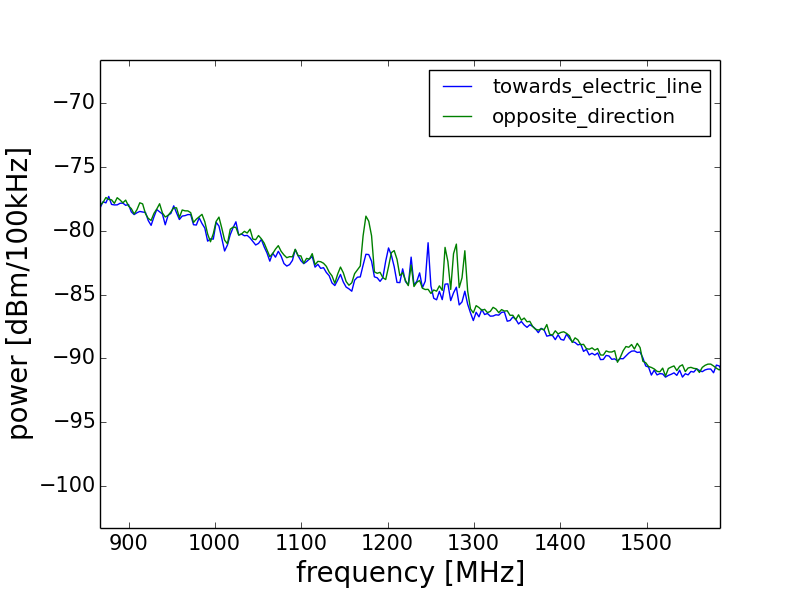
\includegraphics[width=0.49\linewidth]{linecomparison2.png}}
  \caption{spectra with and without filter close to the tank Santy}
  \label{fig:filter}
\end{figure}
\\As  for the  electric line,  we  recorded spectra  with the  antenna
pointed  either toward  the line  (in blue  in Figure~\ref{fig:filter}
(right) ) or facing the  opposite direction (in green). No significant
change is observed, so the line does not produce noise on our setup.
\clearpage
\subsection{Installations}
After the preliminary tests we drove  to all the tanks we will install
an  helix   detector,  i.e.   the   hexagon  centered  on   Santy  (cf
Figure~\ref{fig:hexagon}).    We  took   the   opportunity  that   day
(2016/12/07) to  install two antennas:  Santy and Jorge. The  next day
(2016/12/08) we installed the other antennas in the morning. The order
we proceed  is the  following: Rula, Nono,  Gringa, Gilda,  Eva.\\ The
procedure for the installation is:
\begin{itemize}
\item install the antenna on the support (which was left from the first installation)
\item install the electronics box
\item record a spectrum
\item record waveforms with the Picoscope
\item connect the signal to the UB
\end{itemize}
\textbf{remark:    the   adjustable    resistor   setting    was   not
  modified}\\  The  table~\ref{tab:boxnumber}  reports on  the  device
number  installed (antenna,  LNA,  adaptation box).   A more  detailed
description  of   the  measurements  taken   on  site  can   be  found
in~\cite{measurementsdec2016}.
\begin{table}[!h]
\centering
\caption{installation record}
\label{tab:boxnumber}
\begin{tabular}{ |l|l|l|l|l| }
\hline
tank & date & antenna & LNA & adaptation box \\ \hline \hline
Santy (339) & 07 Dec. & FPV7 & AF8 & box 12 \\ \hline
Jorge (329) & 07 Dec. & FPV8 & AF7 & box 5 \\ \hline
Rula (313) & 08 Dec. (9:20 - 9:40) & FPV4 & AF4 & box 11 \\ \hline
Nono (340) & 08 Dec. (10:05 - 10:30) & FPV6 & AF6 & box 9 \\ \hline
Gringa (328) & 08 Dec. (10:35 - 11:00) & FPV2 & AF2 & box 2 \\ \hline
Gilda (334) & 08 Dec. (11:11 - 11:30) & FPV3 & AF3 & box 3 \\ \hline
Eva (330) & 08 Dec. (11:40 - 12:20) & FPV5 & AF5 & box 10 \\ \hline
\end{tabular}
\end{table}
We  had no  particular issue  during  the installations  and we  spent
approximately 30 minutes  per tank. The pictures of  the antennas once
installed can be found on the Figure~\ref{fig:pics}.\\ \textbf{Remark:
  We went on Gringa  and Nono a second time on the  11th and 12th, see
  section~\ref{sec:update} for more details}
\begin{figure}[ht!]
  \centering
  \hspace*{-3ex}
  \subfigure{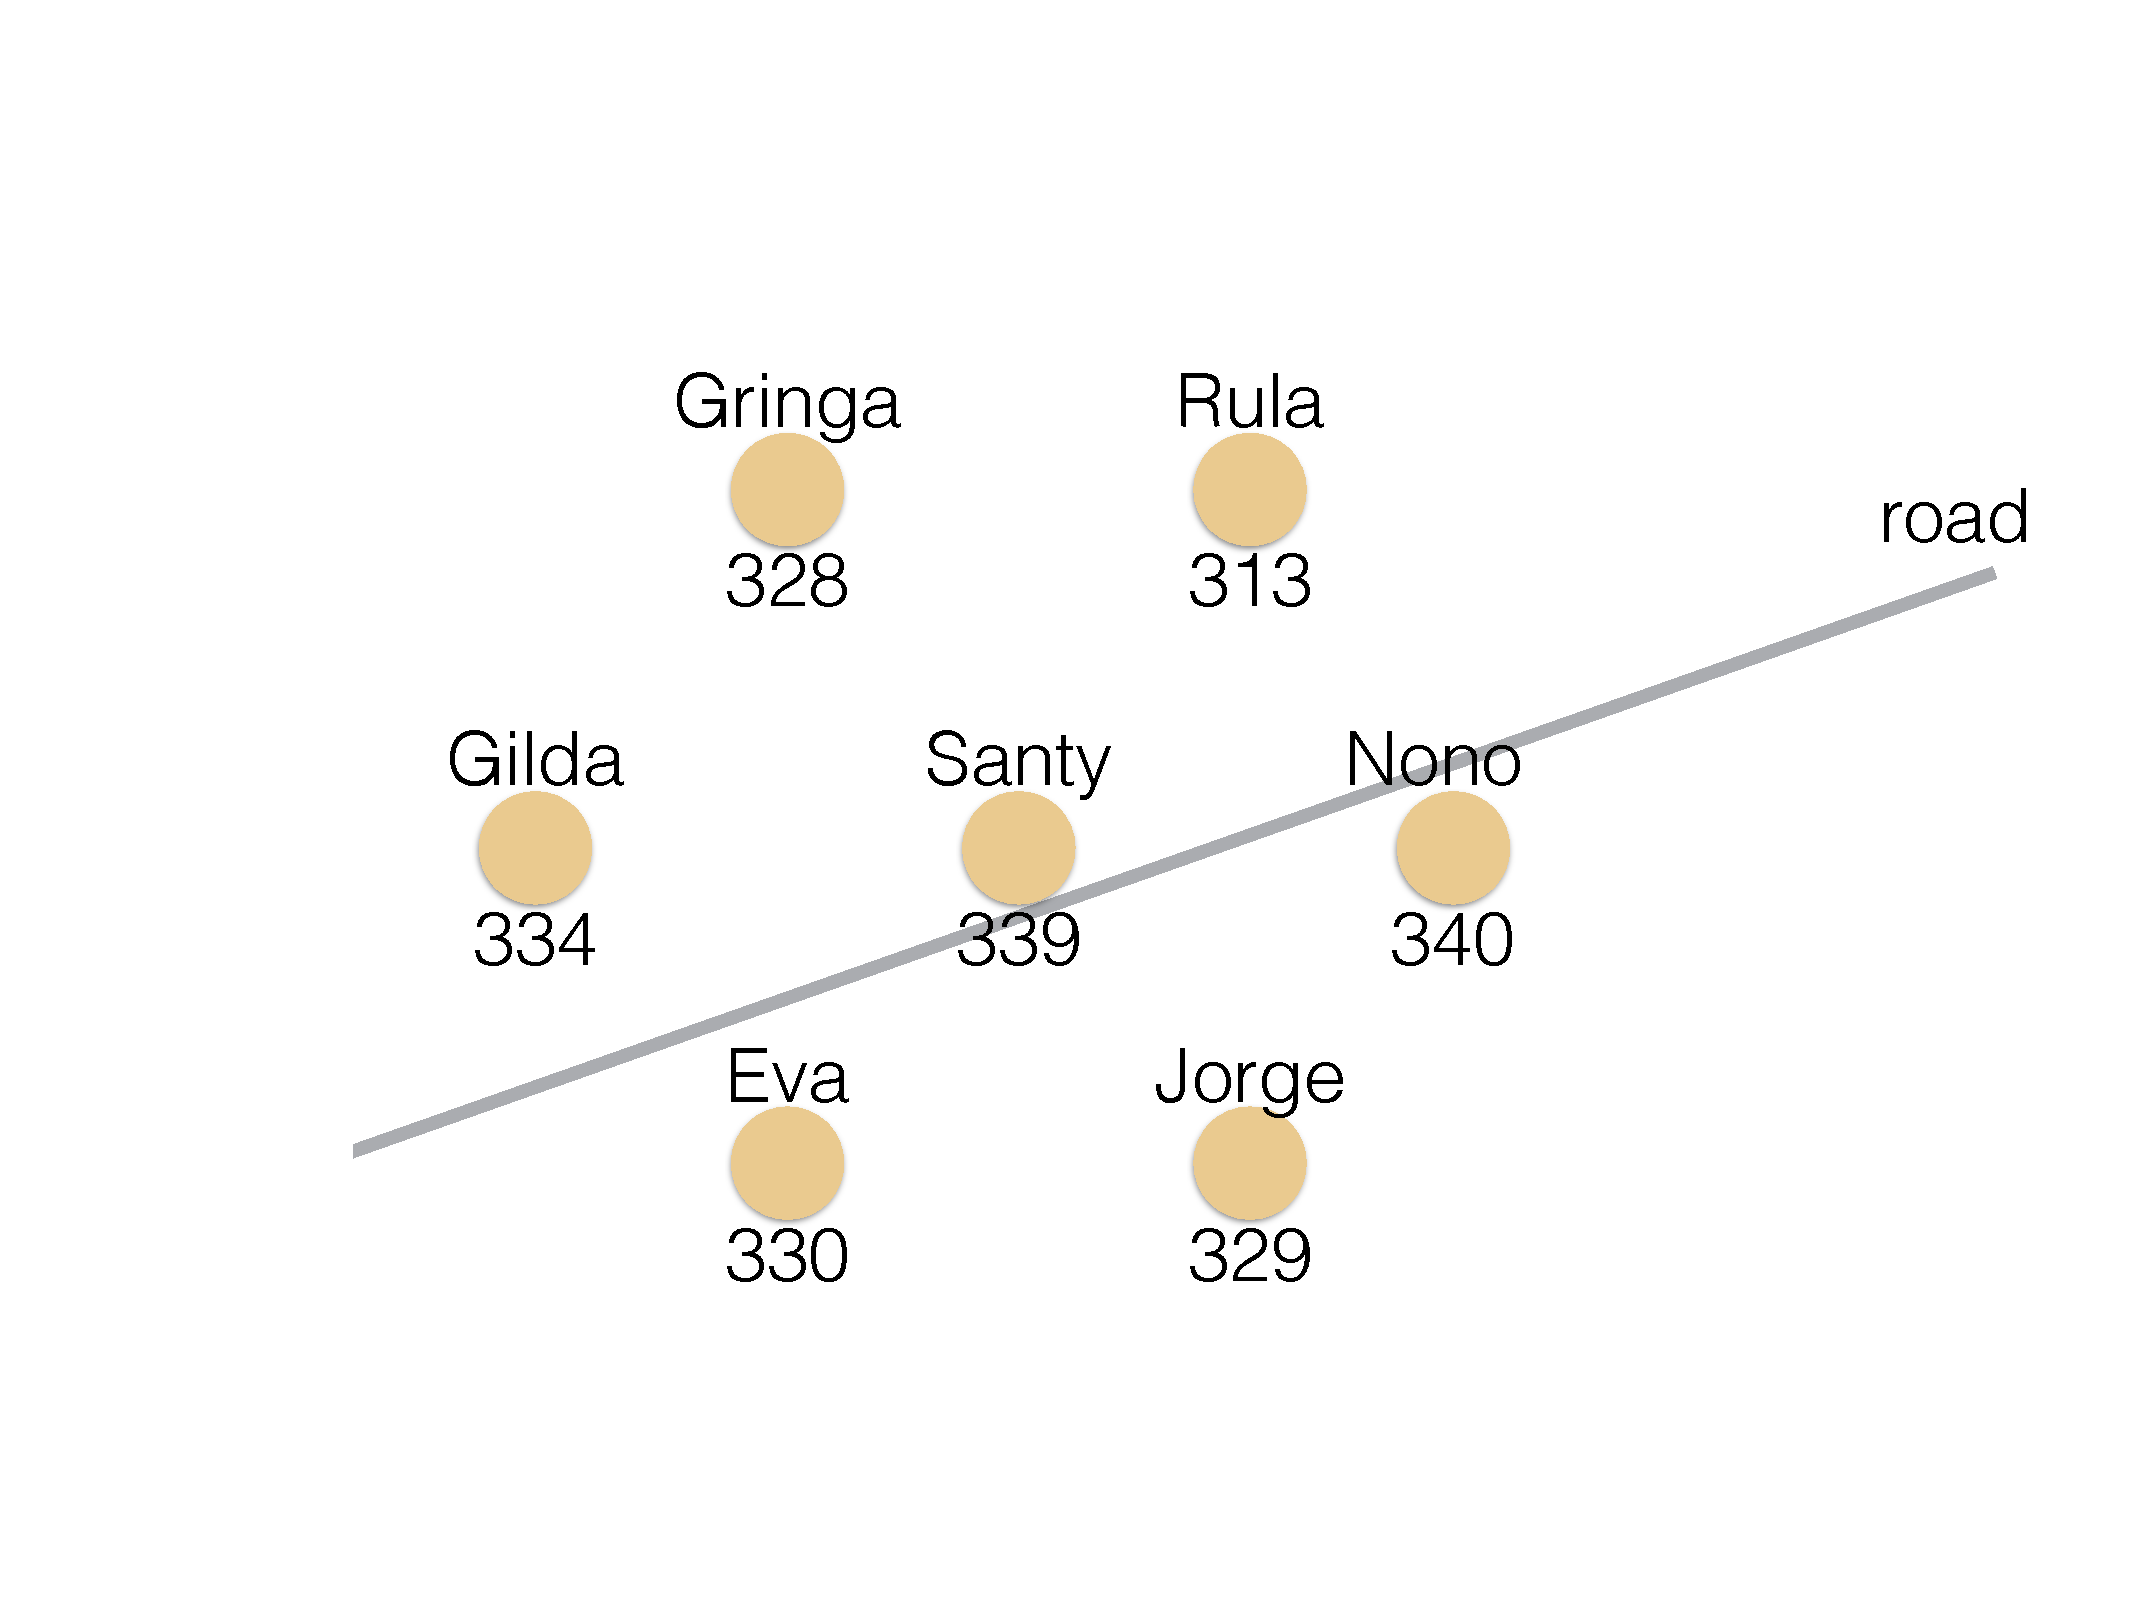
\includegraphics[width=0.70\linewidth]{helixhexagon.pdf}}
  \caption{hexagon where the helix array is installed}
  \label{fig:hexagon}
\end{figure}
\begin{figure}[ht!]
  \centering
  \hspace*{-3ex}
  \subfigure{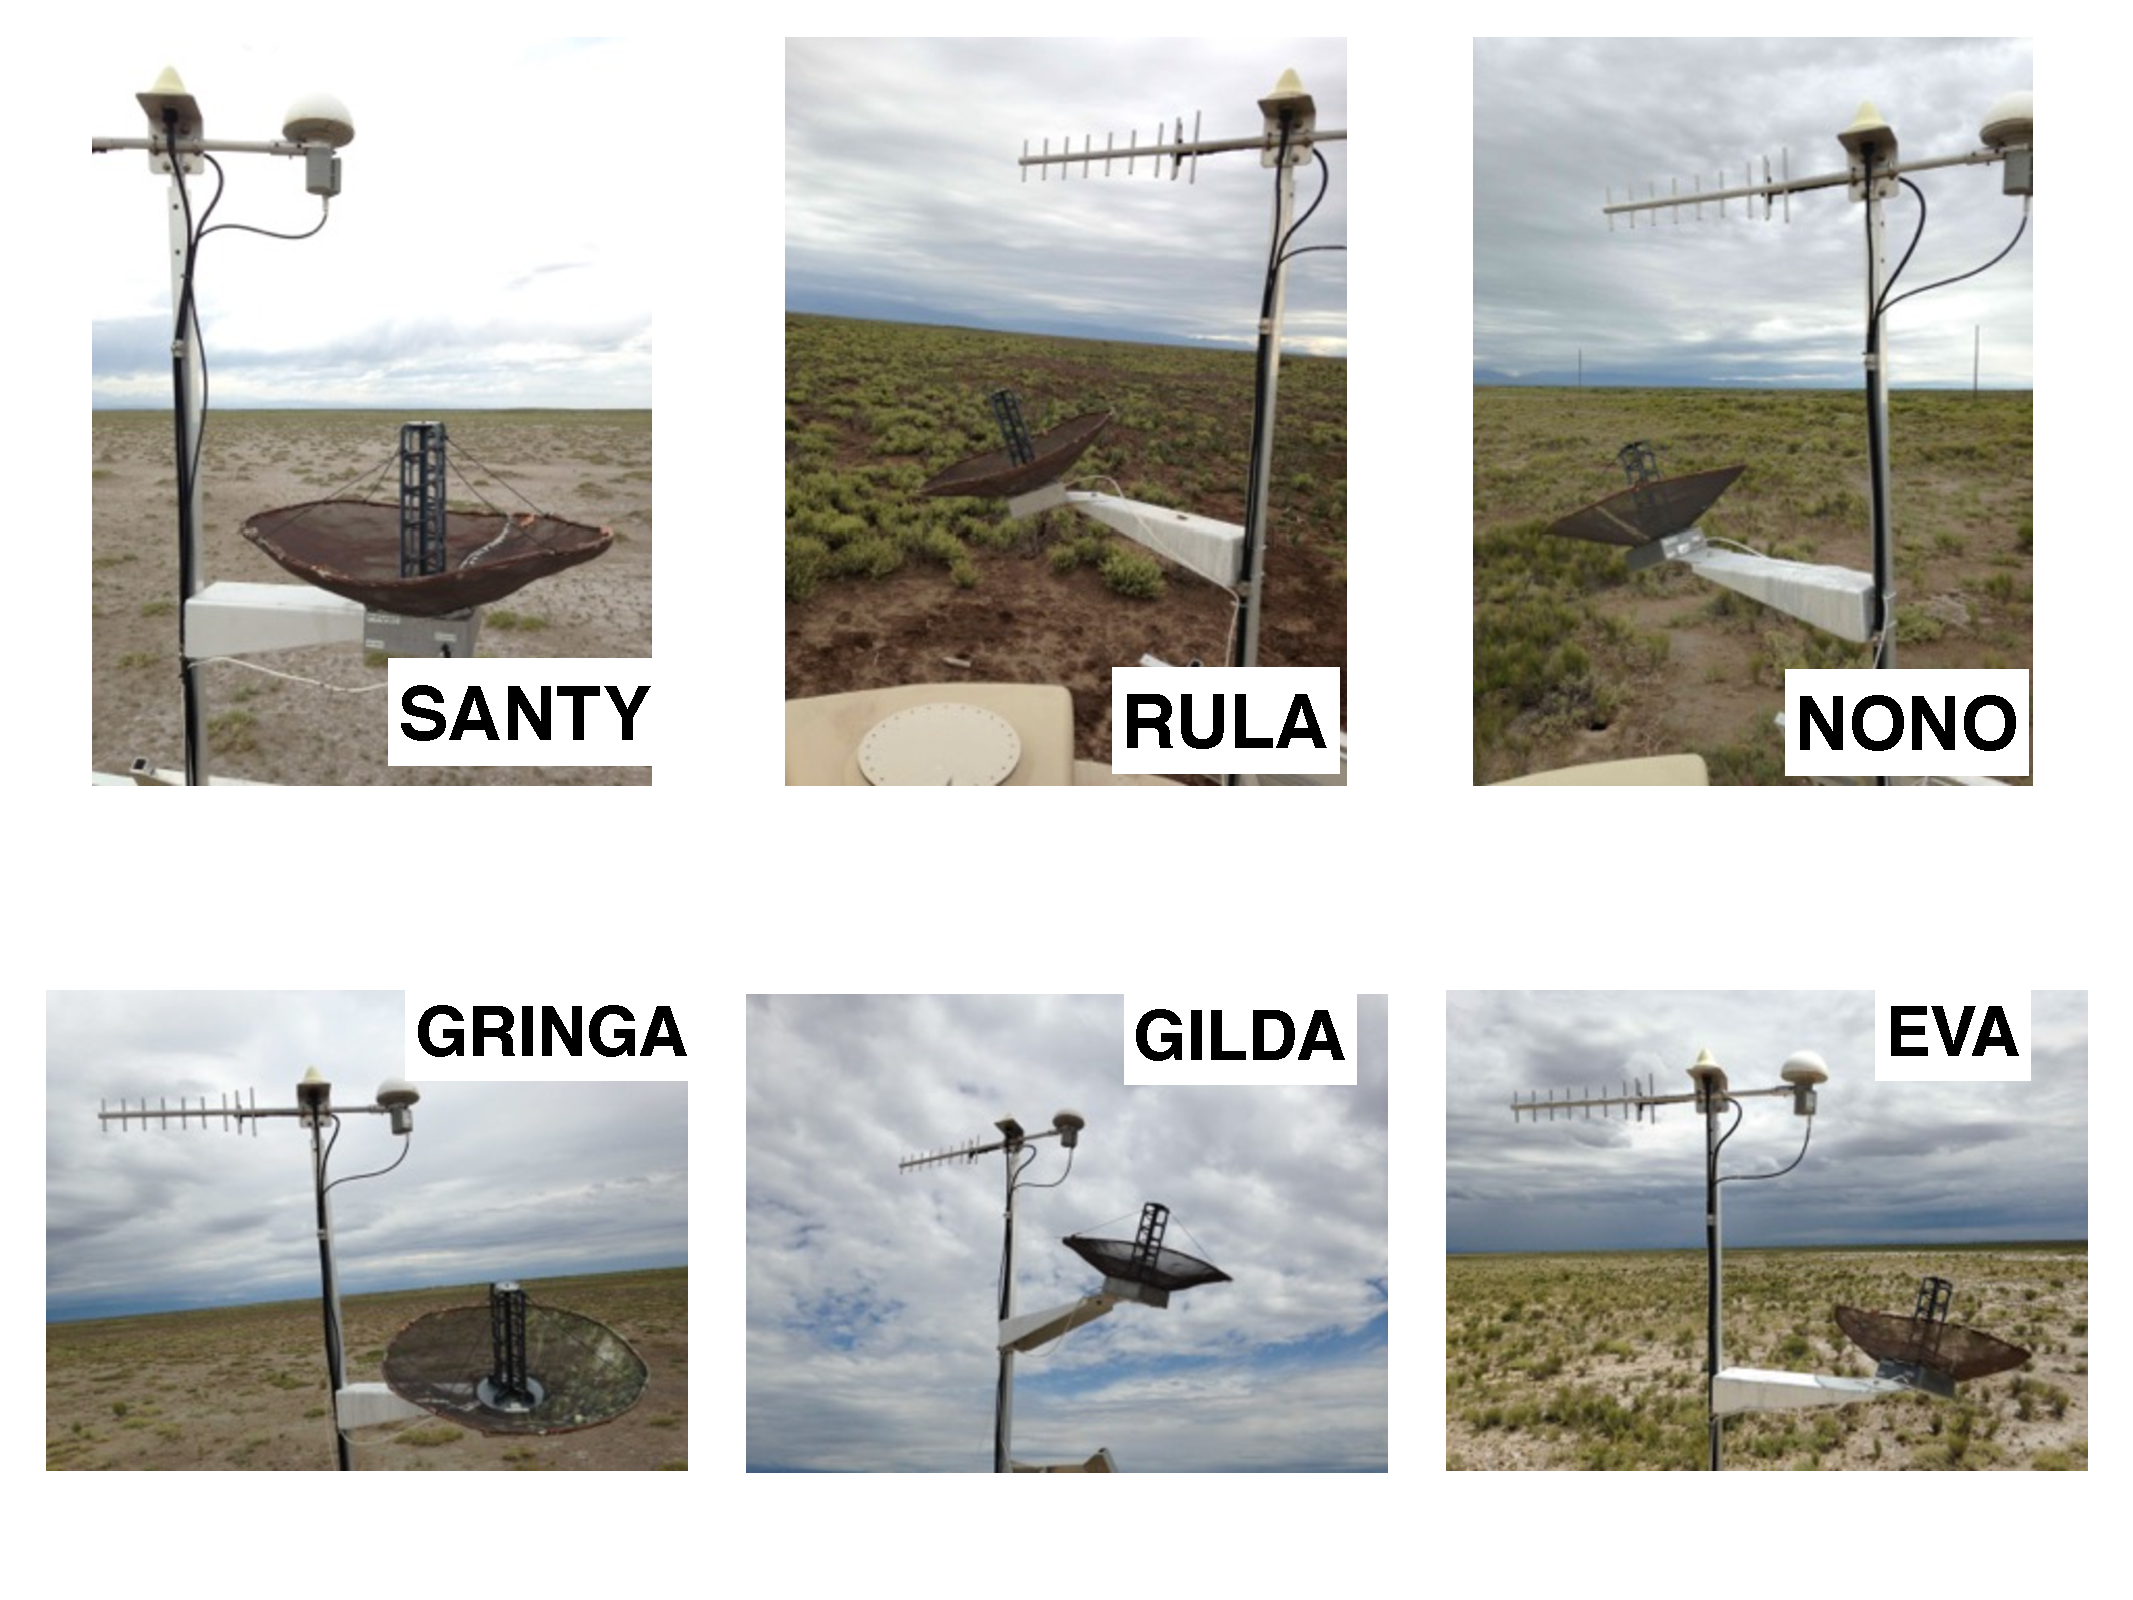
\includegraphics[width=0.70\linewidth]{detpics.pdf}}
  \caption{Picture of all the antennas (except Jorge)}
  \label{fig:pics}
\end{figure}
\clearpage
\section{First observations}
We recorded  data during the  installation to check that  the detector
was operating correctly but also to measure the ambient noise. 
\subsection{spectra}
On all the  tanks we recorded a spectrum, in RMS  mode, to measure the
noise    floor     .    They     are    all    presented     on    the
Figure~\ref{fig:noisefloor}.
\begin{figure}[ht!]
  \centering
  \hspace*{-3ex}
  \subfigure{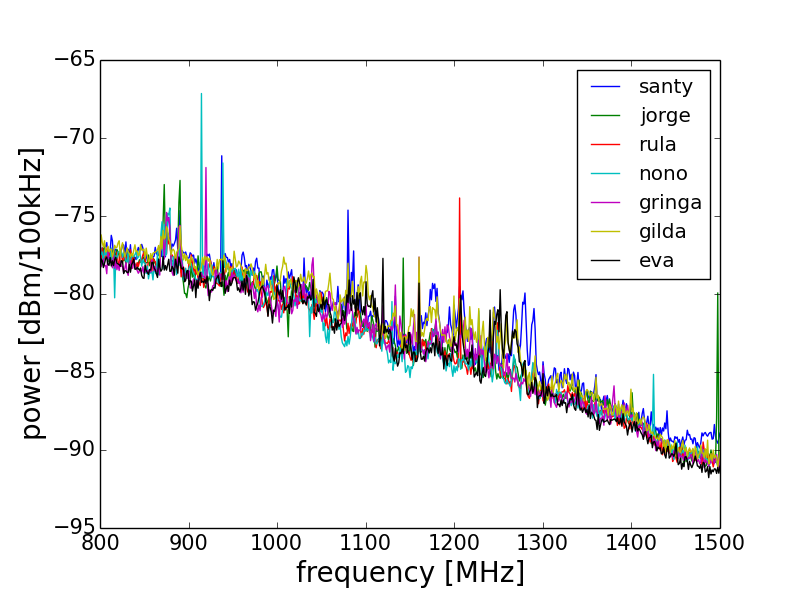
\includegraphics[width=0.7\linewidth]{noisefloor.png}}
  \caption{spectra in RMS mode on all the 7 detectors installed}
  \label{fig:noisefloor}
\end{figure}
\begin{figure}[ht!]
  \centering
  \hspace*{-3ex}
  \subfigure{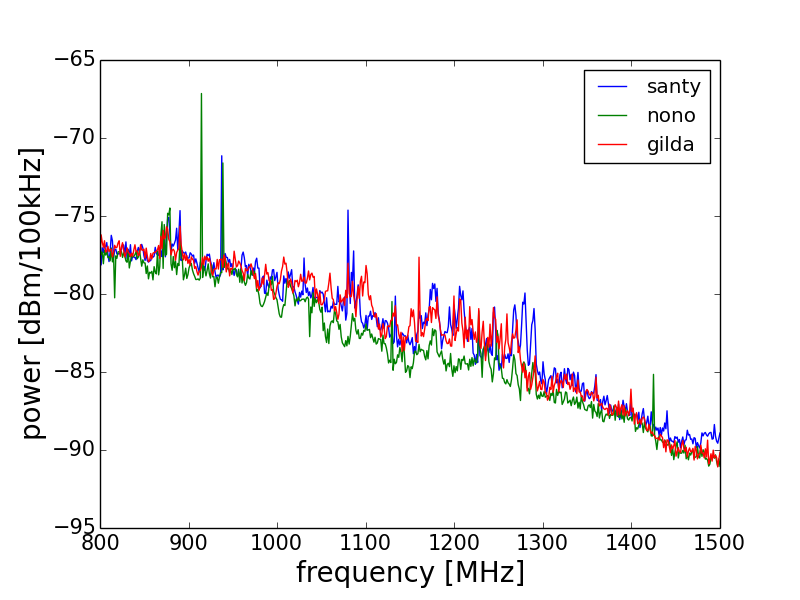
\includegraphics[width=0.49\linewidth]{closetoline.png}}
  \subfigure{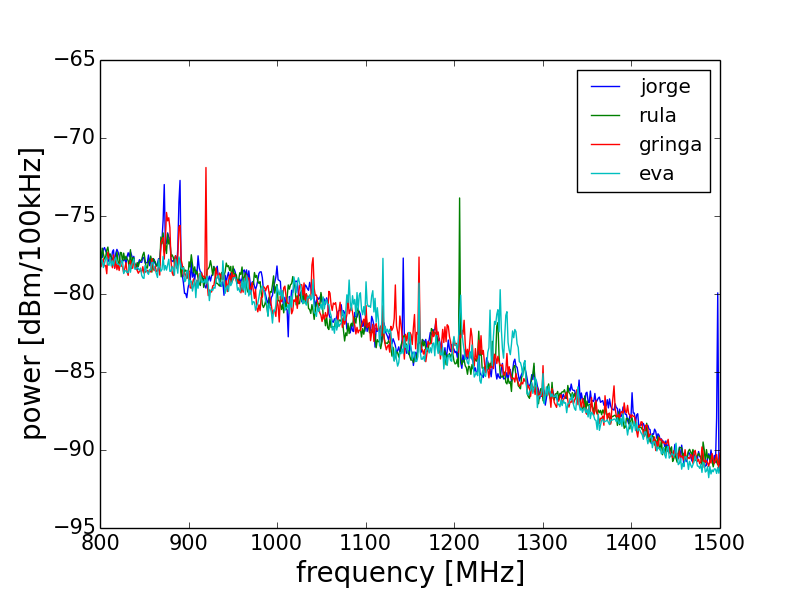
\includegraphics[width=0.49\linewidth]{noline.png}}
  \caption{spectra of detectors close to the line (left) and further away (right)}
  \label{fig:linenoline}
\end{figure}
We see already  on this spectra that there are  peaks inside our band.
With  the  same  data  we  can  also  check  that  the  noise  is  not
significantly larger in  the detectors close to the  electric line (cf
Figure~\ref{fig:linenoline}).\\ We also  recorded spectra in peak mode
but only for the five detectors  installed on the second day.  We show
in Figure~\ref{fig:specpeak} for each  detector approximately 15 to 30
spectra recorded consecutively. The  spectra recorded on Rula and Nono
were taken  with 20dB of attenuation  because the peak  from the Auger
radio  (940MHz) was to  large and  was causing  the saturation  of the
spectrum analyser.   As a result, on  those two detectors  we see less
peaks but this is probably due to the spectrum analyzer attenuation.
\begin{figure}[ht!]
  \centering
  \hspace*{-3ex}
  \subfigure{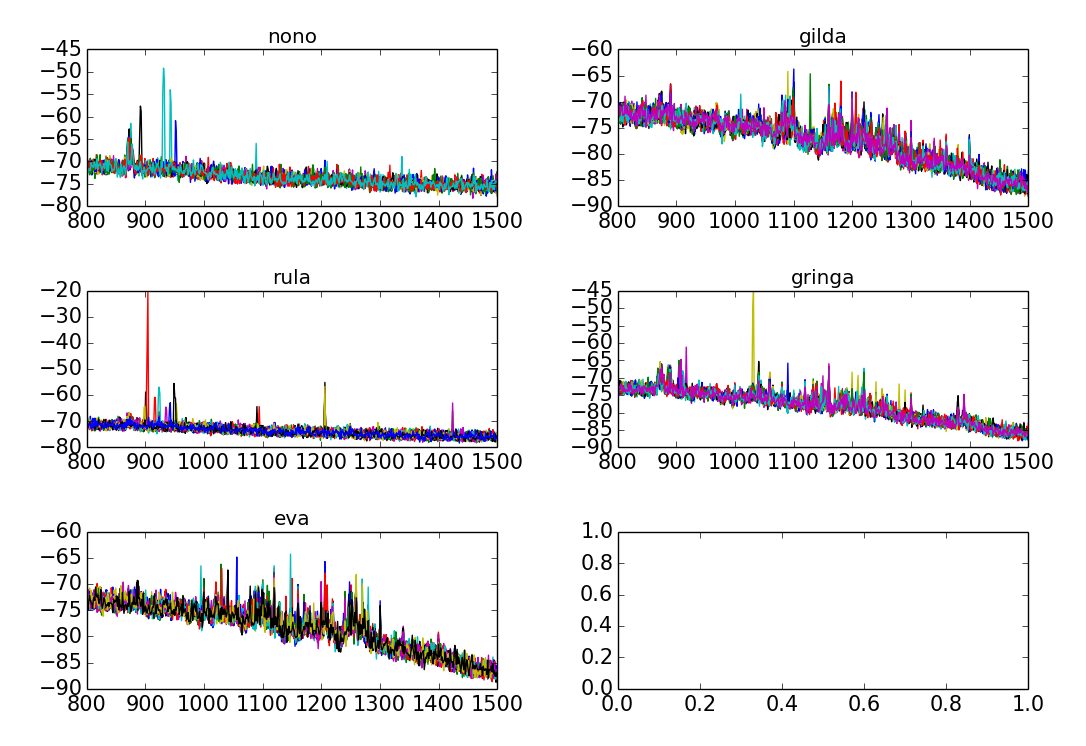
\includegraphics[width=0.7\linewidth]{specpeak.png}}
  \caption{spectra taken in peak mode}
  \label{fig:specpeak}
\end{figure}
It seems that  there are peaks in our band, they  are not obvious when
spectra are taken in RMS mode (Figure~\ref{fig:noisefloor}) but appear
consistently when spectra are acquired in peak mode.


\subsection{waveform}
We also recorded  waveform with the Picoscope. An  example of a 20$\rm
\mu s$ long waveform recorded on Rula is shown in the Figure~\ref{fig:wf}.
\begin{figure}[ht!]
  \centering
  \hspace*{-3ex}
  \subfigure{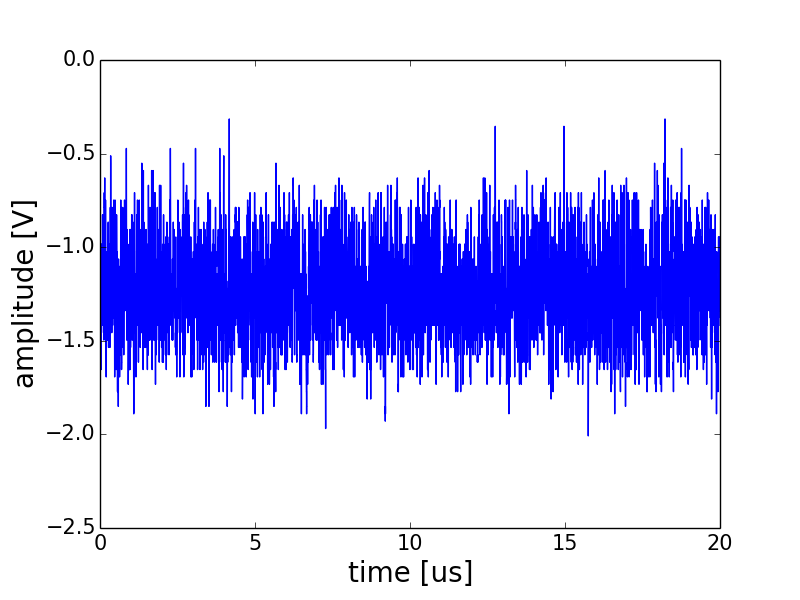
\includegraphics[width=0.7\linewidth]{traceex.png}}
  \caption{example of a trace recorded on Santy tank}
  \label{fig:wf}
\end{figure}

In the real data, the  waveform is slightly different because there is
a 20MHz filter at the input  of the front end. This measurement allows
us to  measure the baseline and  have an idea of  the transient noise.
The distribution  of the amplitudes of  50 traces of 20$\rm  \mu s$ is
shown in  Figure~\ref{fig:distamp}.  The average baseline  and RMS are
reported in table~\ref{tab:baselines}.
\begin{figure}[ht!]
  \centering
  \hspace*{-3ex}
  \subfigure{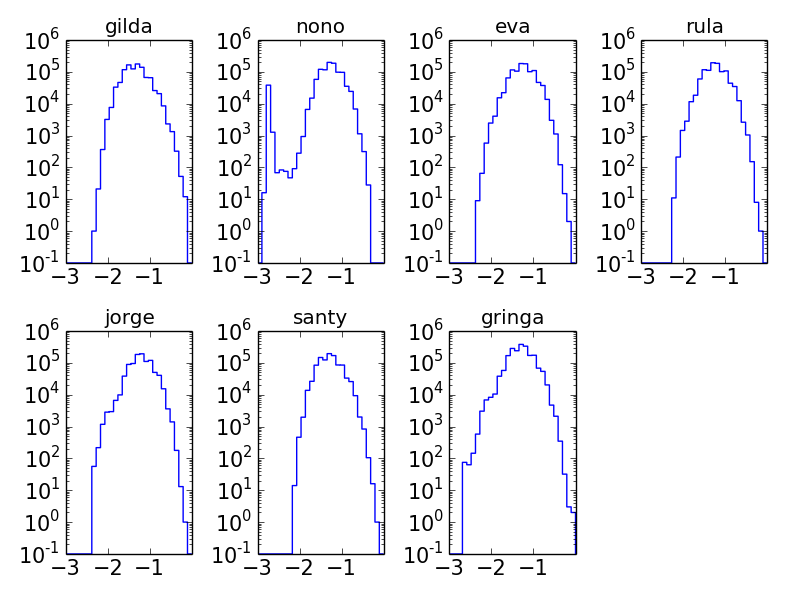
\includegraphics[width=0.7\linewidth]{distamp2.png}}
  \caption{distribution of amplitudes, voltage in x axis and entries in y axis}
  \label{fig:distamp}
\end{figure}

\begin{table}[!h]
\centering
\caption{average value of amplitude  (mean of the distributions of the
  fig~\ref{fig:distamp}), standard deviation on  the average of the 50
  traces recorded and standard deviation of the distribution }
\label{tab:baselines}
\begin{tabular}{ |l|l|l|l|l|l|l|l| }
\hline
tank & santy & jorge & rula & nono & gringa & gilda & eva \\ \hline \hline 
mean [V] & -1.285 & -1.210 & -1.245 & -1.396 & -1.293 & -1.341 & -1.243 \\ \hline
std(mean) [V] & 0.001 & 0.007 & 0.011 & 0.23 & 0.003 & 0.002 & 0.007\\ \hline
rms [V]  & 0.236 & 0.238 & 0.239 & 0.358 & 0.256 & 0.254 & 0.250\\ \hline
\end{tabular}
\end{table}
For all the antennas, the baseline is around -1.3V but their amplitude
distributions  have a different  shape.  Especially  Nono has  a large
contribution at around -3V, Gringa or  Jorge have also a tail at large
negative value.  The tail in  the distribution can be explained by the
presence of transient noise. This is confirmed by the triggered traces
we recorded on  Jorge.  Some examples of these  waveforms are shown in
Figure~\ref{fig:transient}.
\begin{figure}[ht!]
  \centering
  \hspace*{-3ex}
  \subfigure{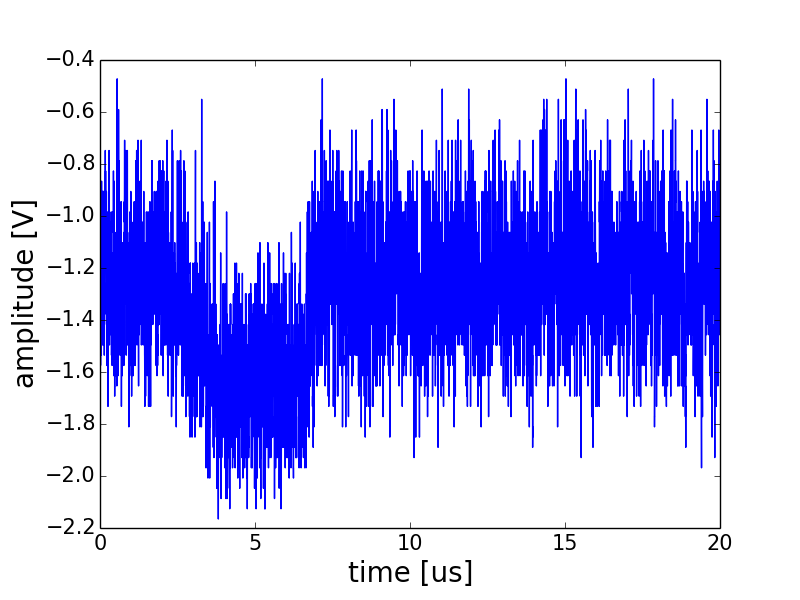
\includegraphics[width=0.32\linewidth]{transientshort.png}}
  \subfigure{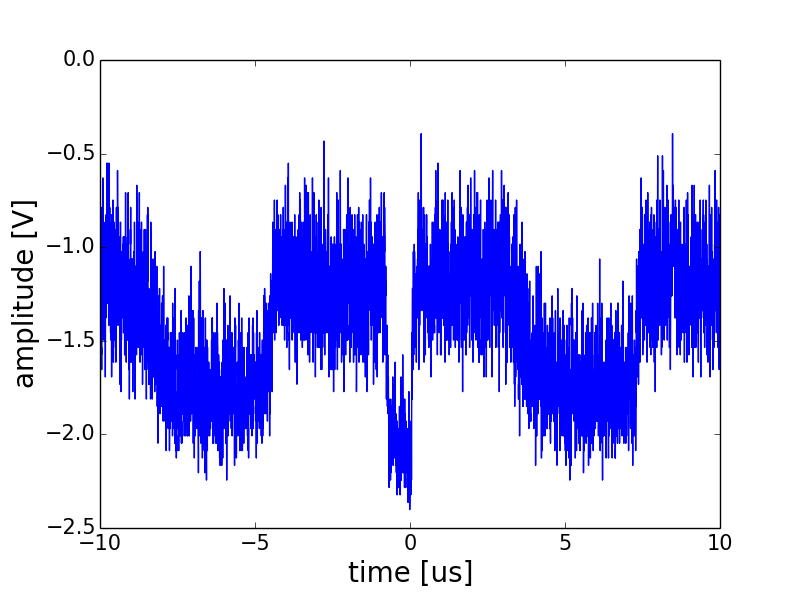
\includegraphics[width=0.32\linewidth]{transientshort2.png}}
  \subfigure{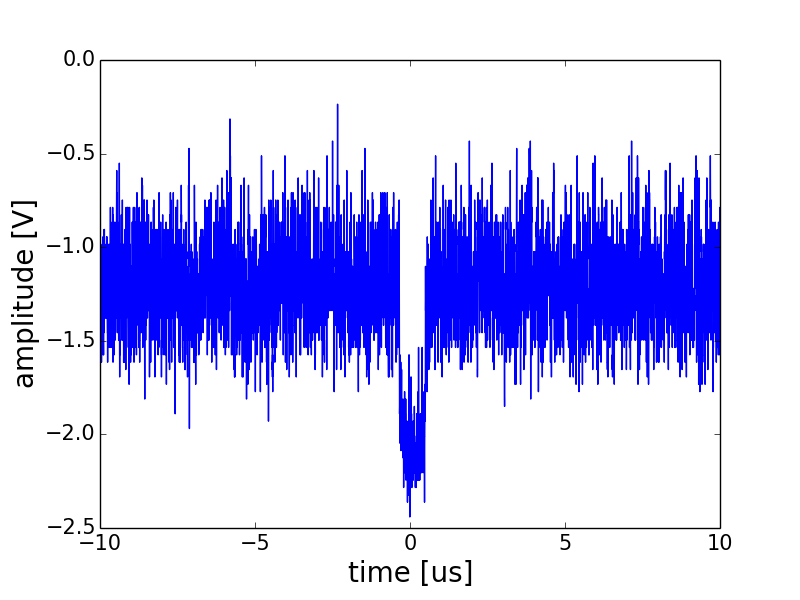
\includegraphics[width=0.32\linewidth]{transientshort3.png}}
  \caption{}
  \label{fig:transient}
\end{figure}

By looking  at longer waveform (of  the order of the  second), see for
instance  Figure~\ref{fig:longwf},  we see  a  strong transient  noise
every second  in the  case of  Nono.  It appears  also in  Gringa, and
probably in  Rula (but I lost  the file...).  This  peak appears every
second and  is 10ms long.  This  noise is very likely  coming from the
Auger  comms.  The  waveform and  spectra of  Gilda and  Eva  are much
cleaner.
\begin{figure}[ht!]
  \centering
  \hspace*{-3ex}
  \subfigure{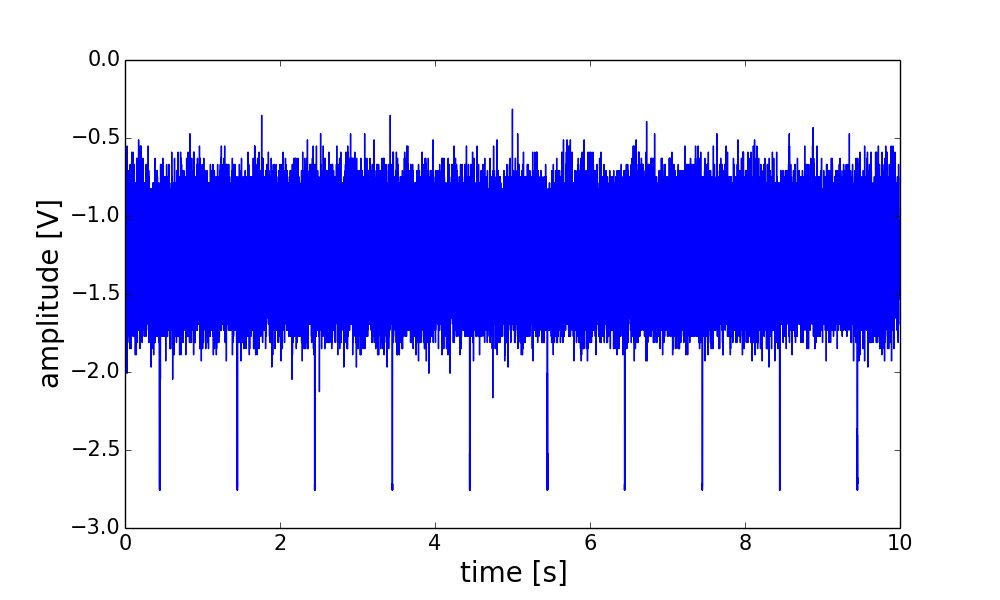
\includegraphics[width=0.49\linewidth]{longtracenono.png}}
  \subfigure{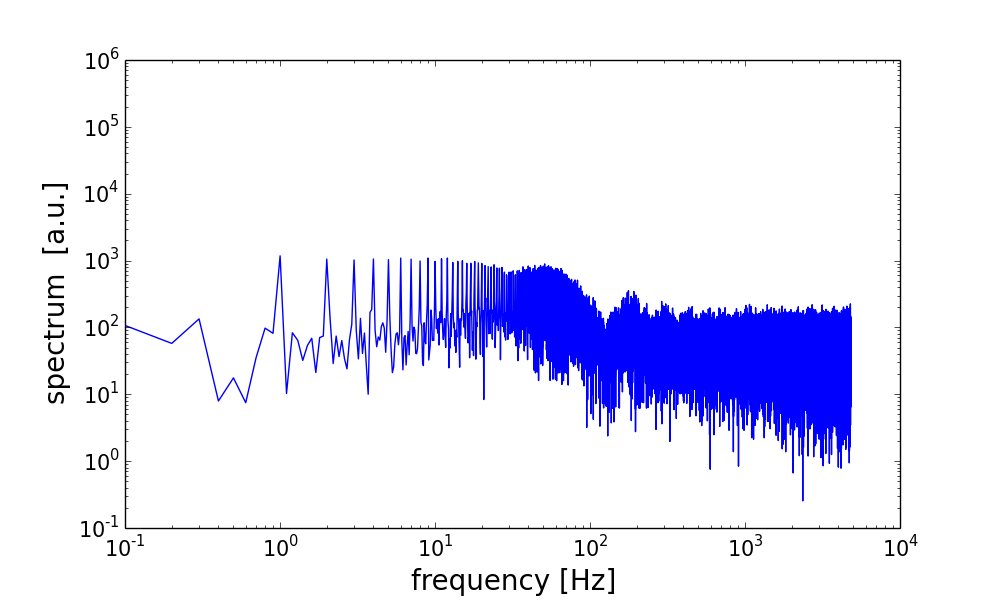
\includegraphics[width=0.49\linewidth]{longspecnono.png}}\\
  \subfigure{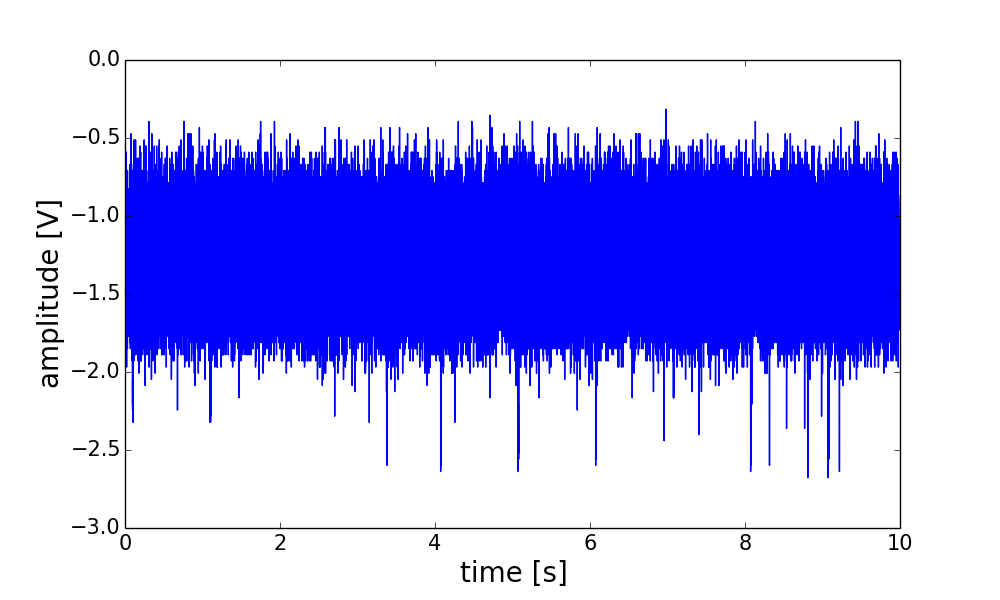
\includegraphics[width=0.49\linewidth]{longtracegringa.png}}
  \subfigure{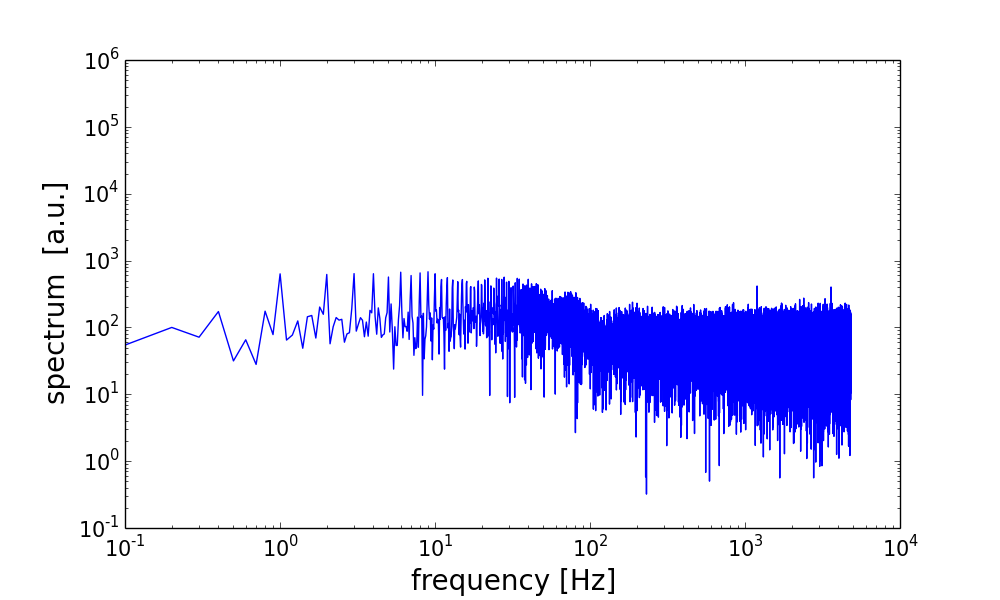
\includegraphics[width=0.49\linewidth]{longspecgringa.png}}\\
  \subfigure{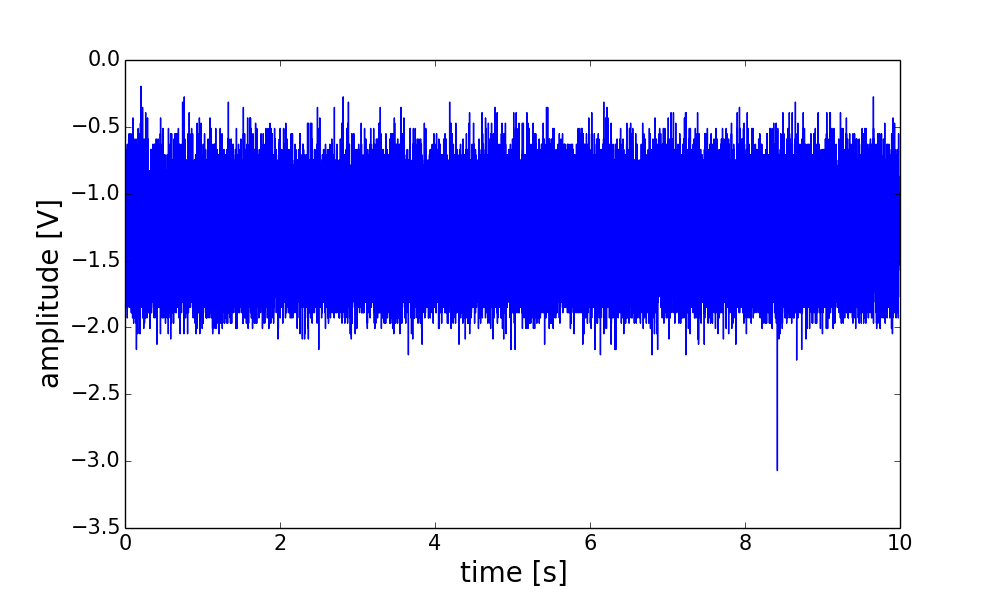
\includegraphics[width=0.49\linewidth]{longtracegilda.png}}
  \subfigure{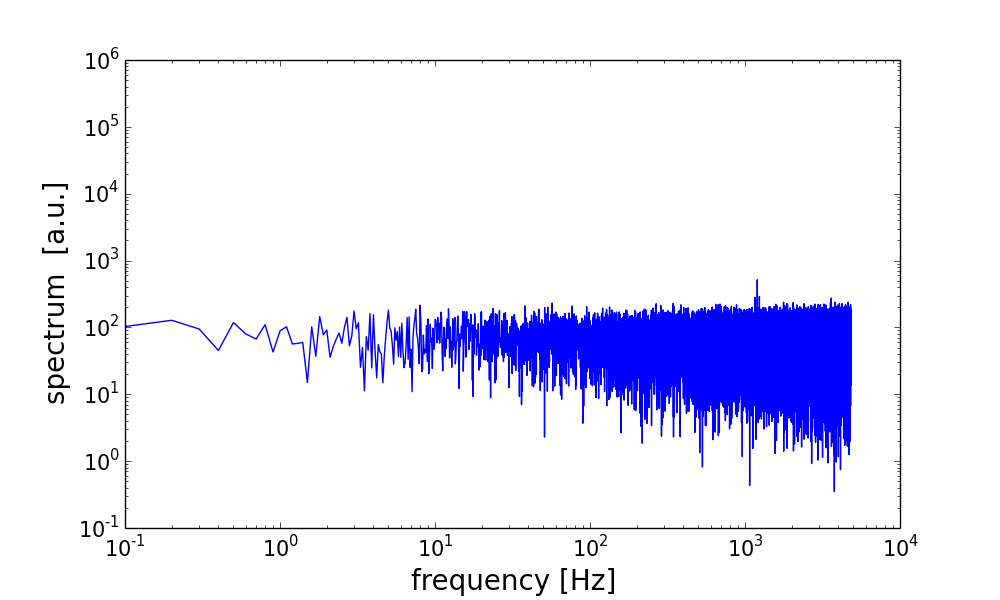
\includegraphics[width=0.49\linewidth]{longspecgilda.png}}\\
  \subfigure{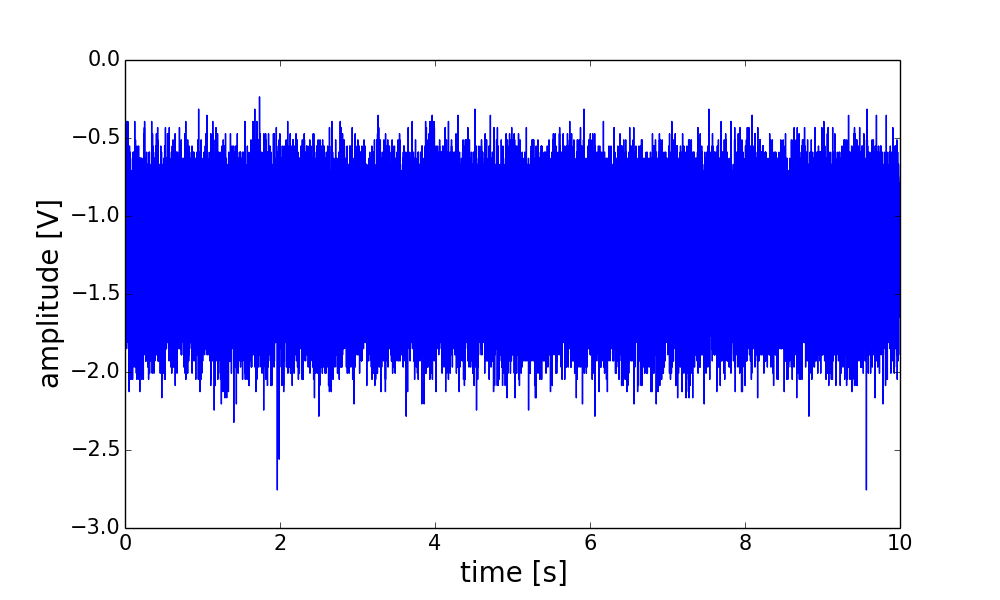
\includegraphics[width=0.49\linewidth]{longtraceeva.png}}
  \subfigure{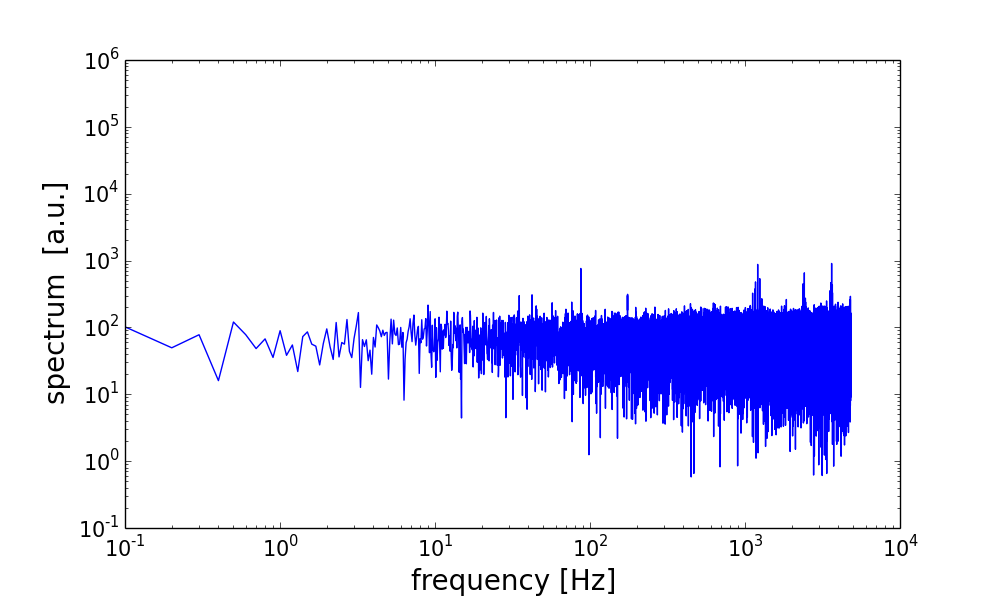
\includegraphics[width=0.49\linewidth]{longspeceva.png}}
  \caption{from top to bottom: Nono, Gringa, Gilda, Eva}
  \label{fig:longwf}
\end{figure}



\clearpage
\subsection{monitoring}
The   baseline  can  be   checked  with   the  monitoring   data,  see
Figure~\ref{fig:monit}.   Firstly,  we  see  that the  baseline  value
matches  the baseline  voltage  measured with  the  picoscope on  site
(650ADC count correspond to  around -1.3V).  Unfortunately we see that
Gringa seem  to be  broken. This might  be due  to a strong  wind that
occured during the  night 9th to the 10th and during  the whole day of
the 10th.   \\We can also note  that the baseline varies  less than in
the C-band, there seem to be less temperature dependence.  \\The helix
antennas are tilted toward the center of the hexagon, only the central
detector points toward the zenith.  So we expect different signal from
the sun depending  on the antenna. In this season, we  expect to see a
bump  from the  sun  in five  antennas  (all of  them  except the  two
pointing toward the  south: Rula and Gringa). The  sun is very clearly
visible in  Eva and Gilda.  It  is also visible, but  less clearly, in
Jorge and Santy, however it is  really not obvious in Nono. This means
that Nono is  less sensitive than the other antenna. It  can be due to
the larger transient noise it receives.

\begin{figure}[ht!]
  \centering
  \hspace*{-3ex}
  \subfigure{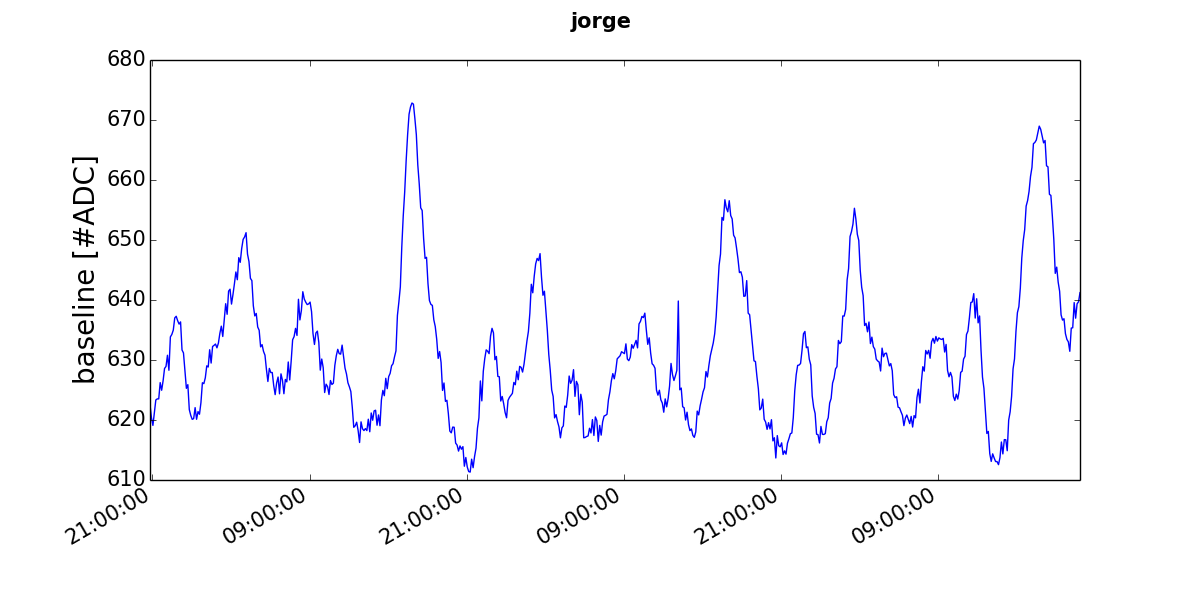
\includegraphics[width=0.49\linewidth]{monitjorge.png}}
  \subfigure{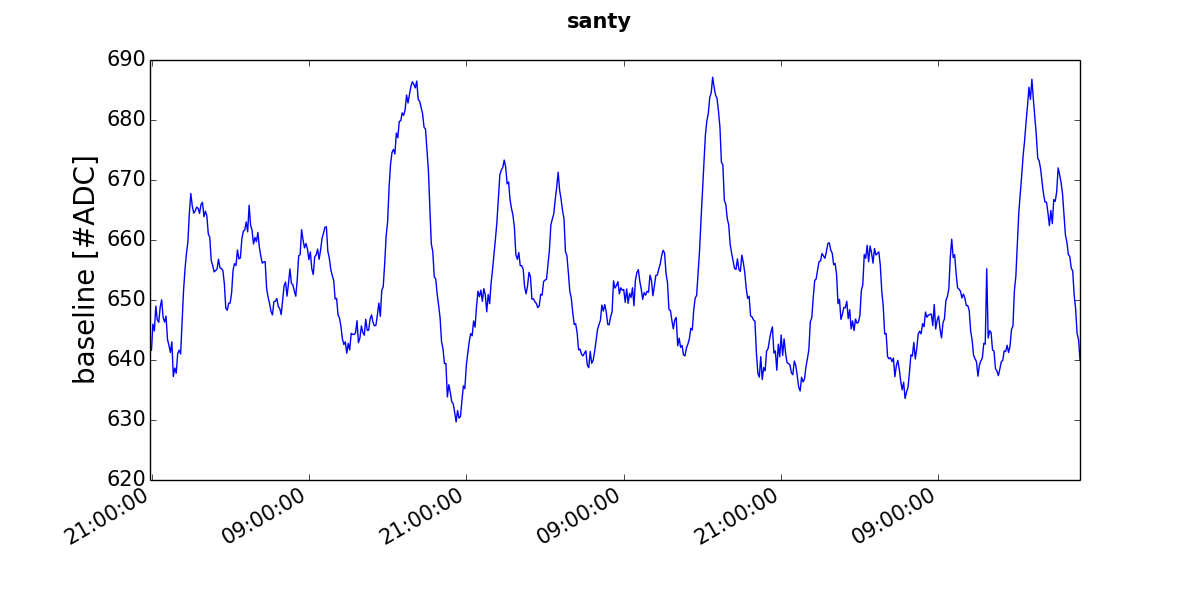
\includegraphics[width=0.49\linewidth]{monitsanty.png}}\\
  \subfigure{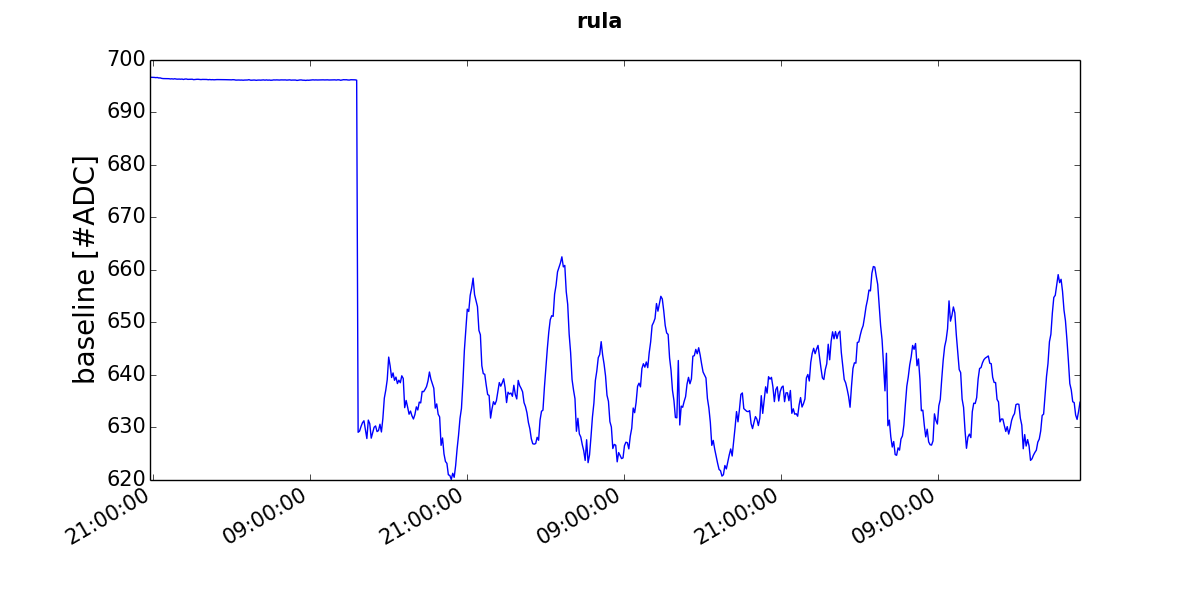
\includegraphics[width=0.49\linewidth]{monitrula.png}}
  \subfigure{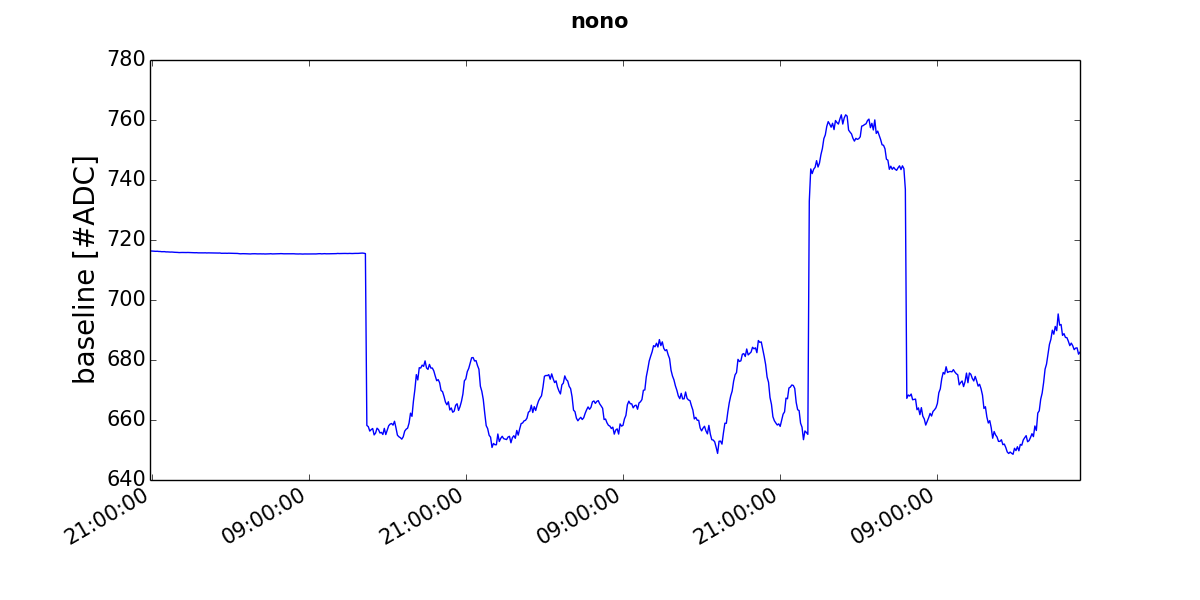
\includegraphics[width=0.49\linewidth]{monitnono.png}}\\
  \subfigure{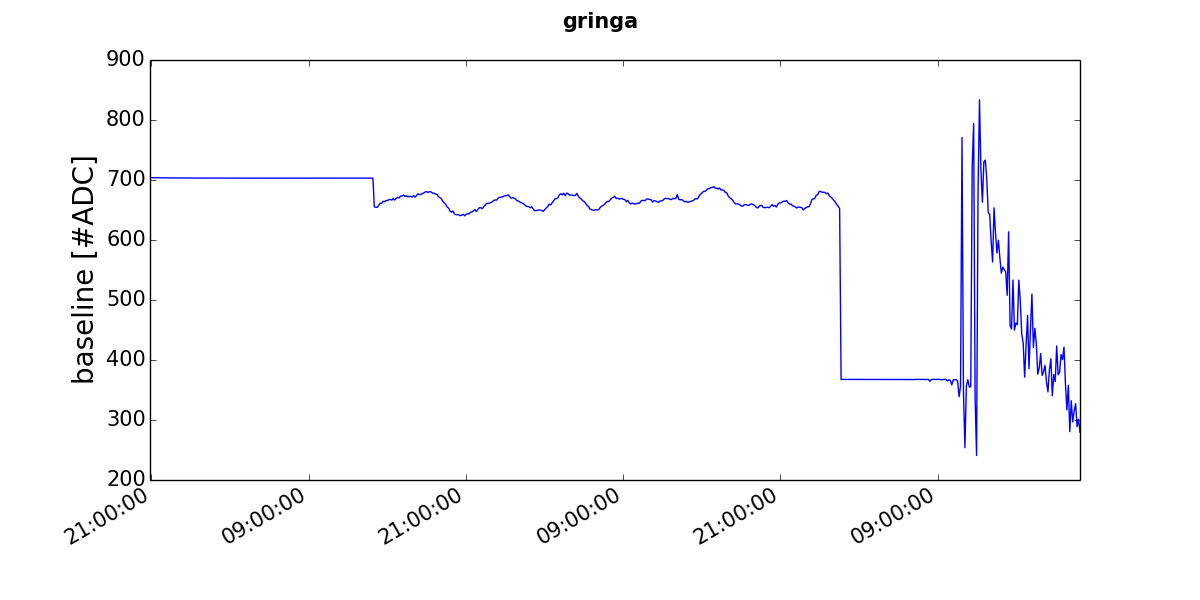
\includegraphics[width=0.49\linewidth]{monitgringa.png}}
  \subfigure{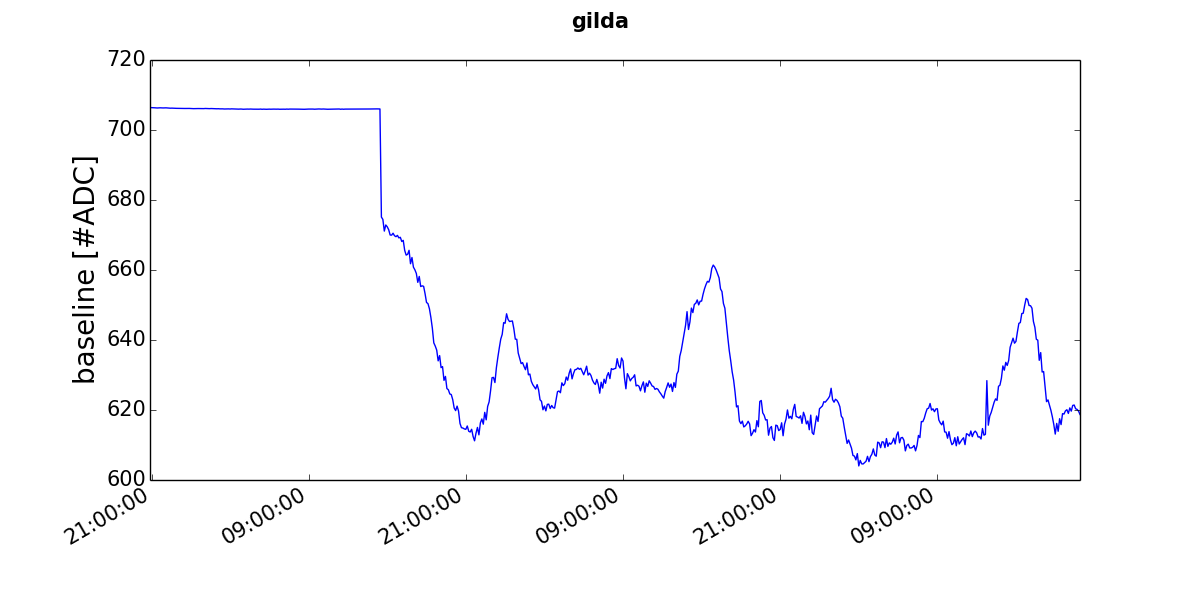
\includegraphics[width=0.49\linewidth]{monitgilda.png}}\\
  \subfigure{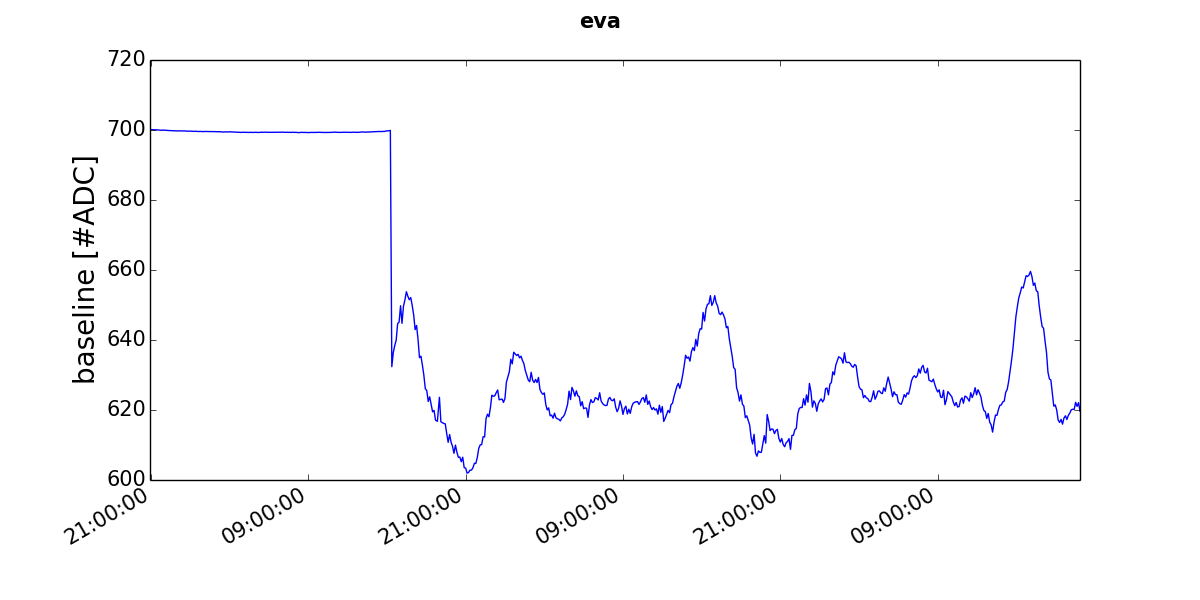
\includegraphics[width=0.49\linewidth]{moniteva.png}}
  \caption{from top to bottom: Nono, Gringa, Gilda, Eva}
  \label{fig:monit}
\end{figure}
\clearpage
\section{Update}
\label{sec:update}
\paragraph{Gringa}
In the previous section we showed that Gringa stopped working on the
10th of the December.  On the 11th we went on site and we spotted the
issue: the adaptation/power distribution board was delivering 24V on
the DC+RF channel instead of 5V (to supply the amplifier).  We got the
antenna and electronics back to the assembly building and we repaired
it.  (We disconnected the DC converter $M3$ and connected the
$V_{out}$ of DC converter $M2$ to the power output at the inductance
$L10$ (see the electronics scheme at~\cite{schemaelec})).\\ From the
monitoring data, it seems to work but it has to be confirmed.
\paragraph{Nono}
We  also noticed  that Nono  seemed to  be less  sensitive  than other
antenna, especially on the sun signal. One of the possible explanation
is the noise produced by the communication antenna which is just above
the antenna on this tank. We  modified the position of the antenna but
we    kept   the    designed   orientation    (see   photo    in   the
Figure~\ref{fig:newnono}. \\From the data we collected on site and the
first monitoring data, no clear improvement is observed.
\begin{figure}[ht!]
  \centering
  \hspace*{-3ex}
  \subfigure{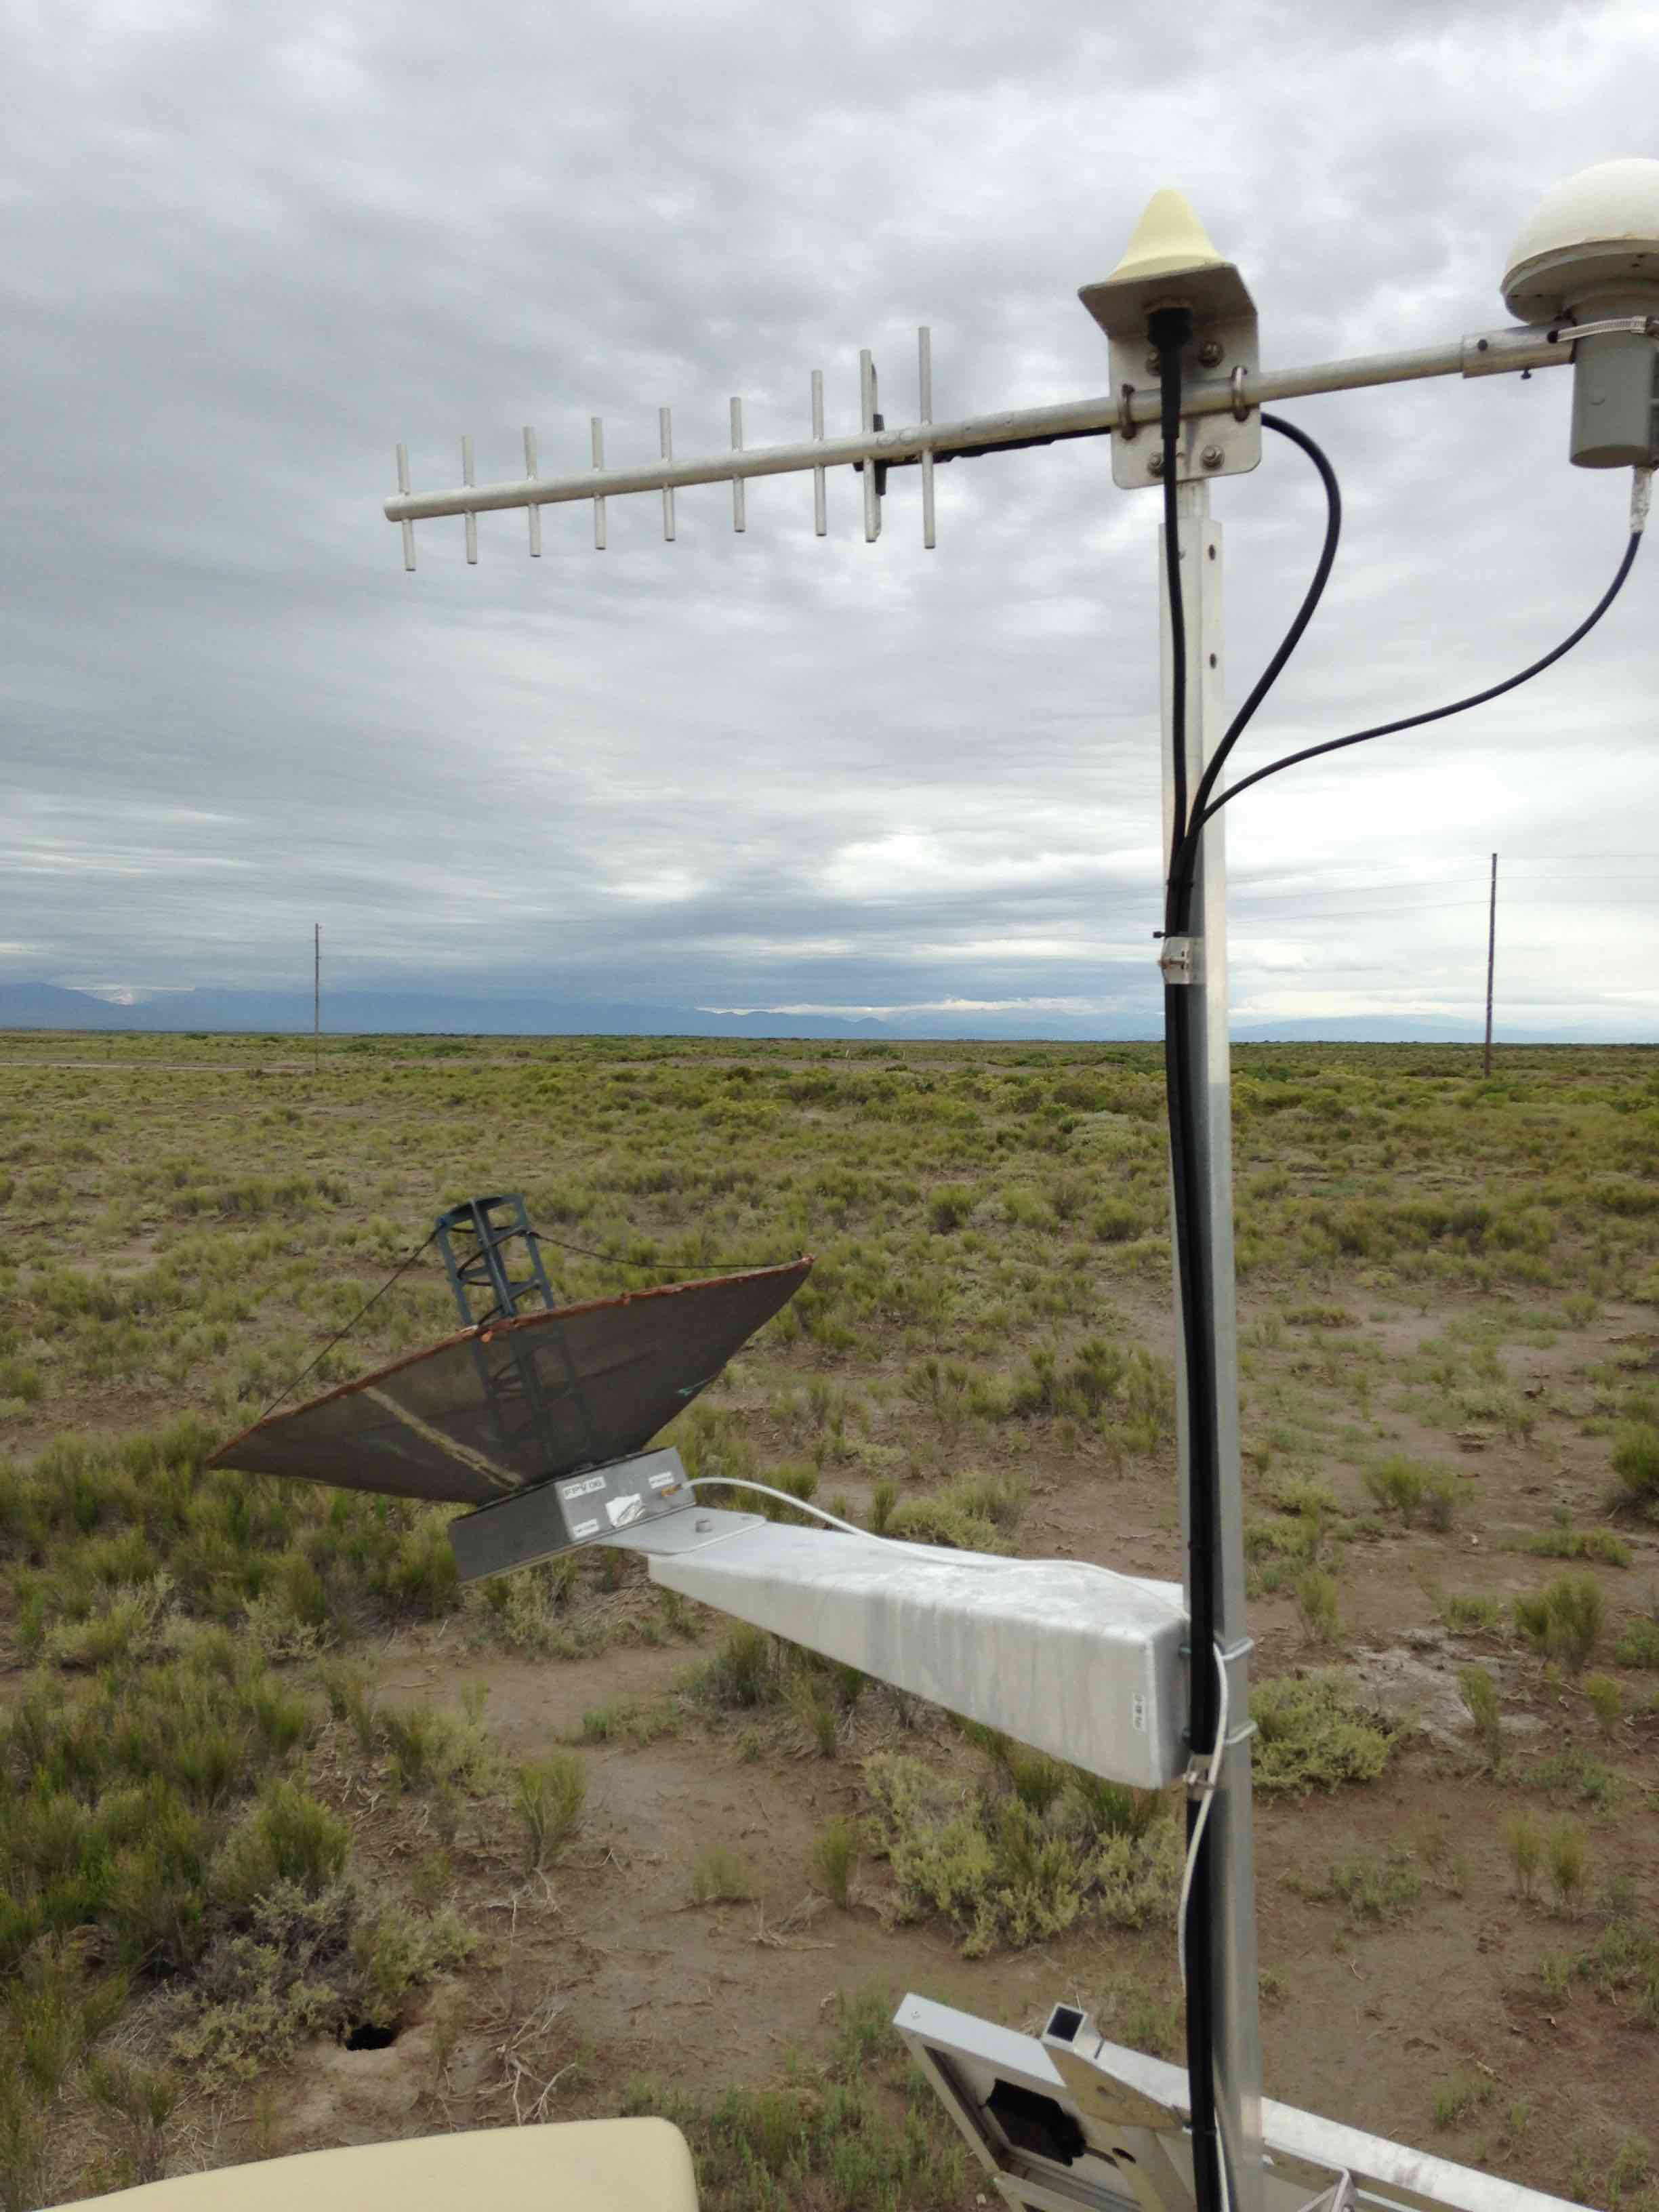
\includegraphics[width=0.49\linewidth]{nono.jpg}}
  \subfigure{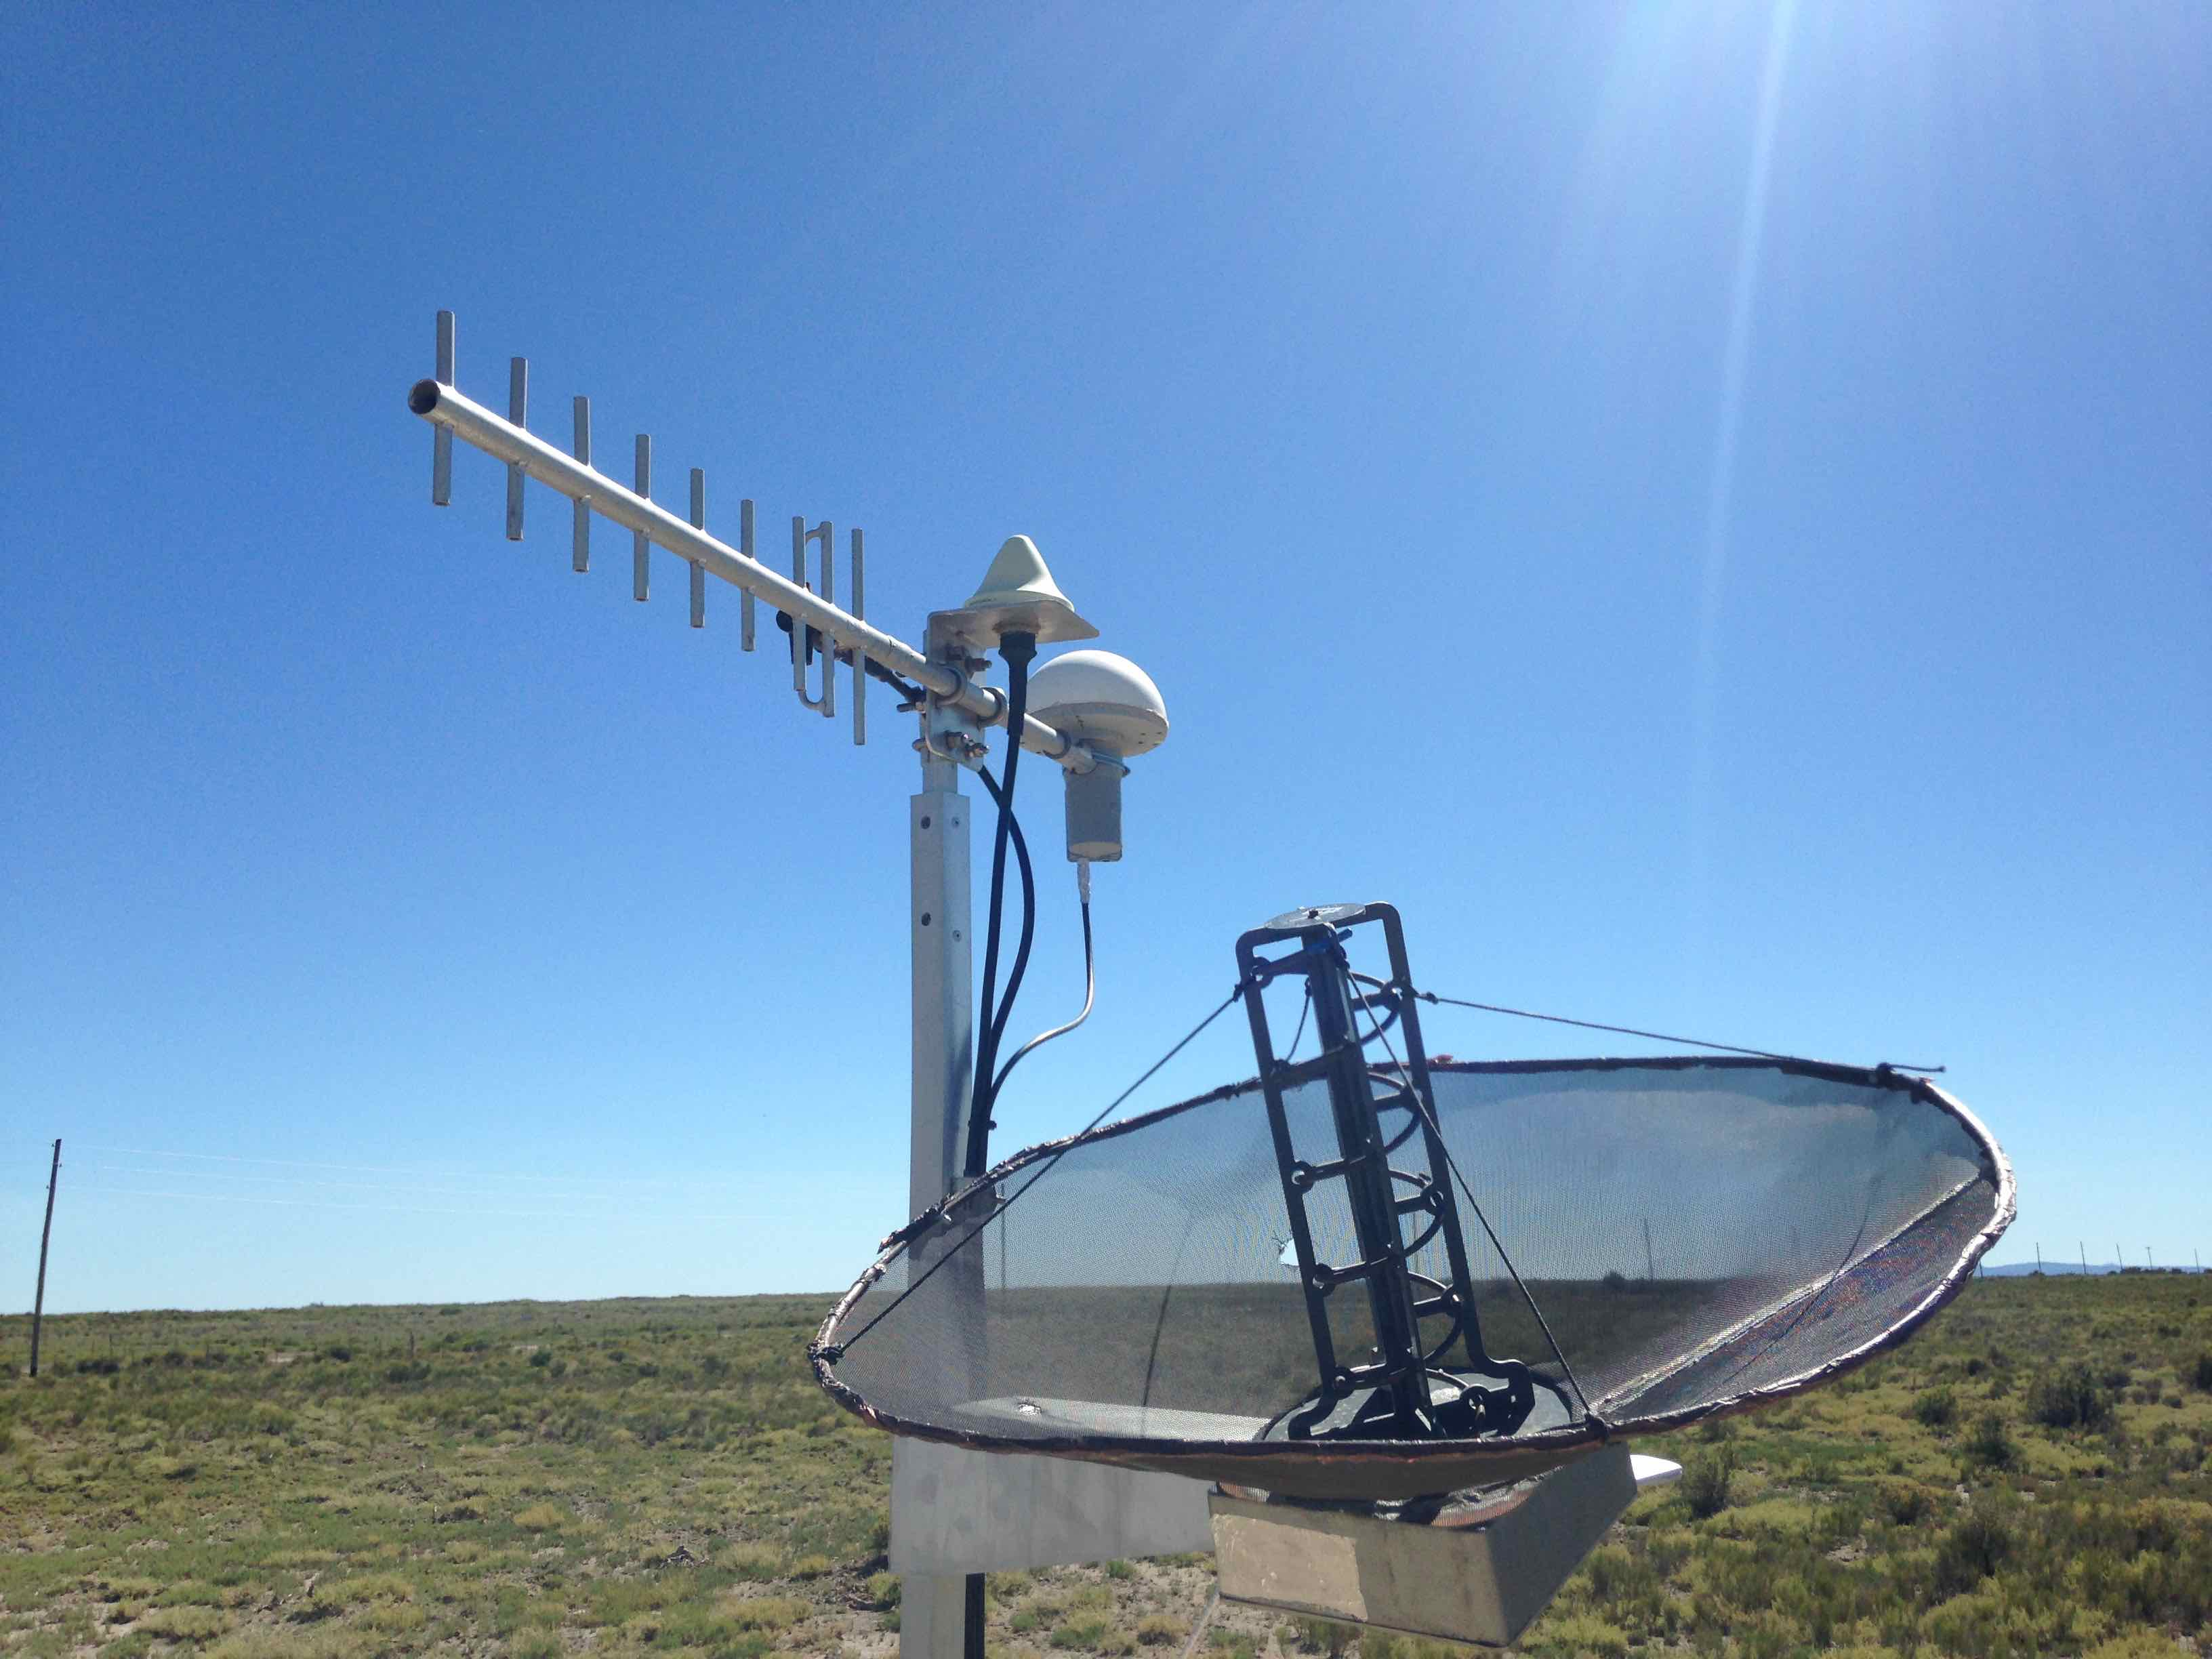
\includegraphics[width=0.49\linewidth]{newnono.jpg}}
  \caption{old and new antenna position on Nono tank}
  \label{fig:newnono}
\end{figure}



\clearpage
\section*{Conclusion (2016/12/12)}
We  installed seven  helix antennas  with the  new  electronics (fixed
adaptation  board  and  new   amplification  system)  on  the  hexagon
initially  chosen (central  tank:Santy). The  installation  took place
from the  7th of December to the  8th and went smoothly.   \\ From the
measurement  taken at  the installation,  we could  conclude  that the
noise floor is  approximately the same for all  the detectors. However
some peaks are observed in the  middle of our frequency band.  We also
observed very clearly a transient noise probably coming from the Auger
communication  link in at  least two  detectors.  \\All  the detectors
worked  just after  being installed.   Gringa  went down  the 10th  of
December but  was repaired and  installed again the 12th.   Nono seems
less sensitive than the other  antennas even after the modification of
its position.  \\A first rough estimation of  system noise temperature
from the sun signal performed  on Jorge yields a temperature of around
100K.
\begin{figure}[ht!]
  \centering
  \hspace*{-3ex}
  \subfigure{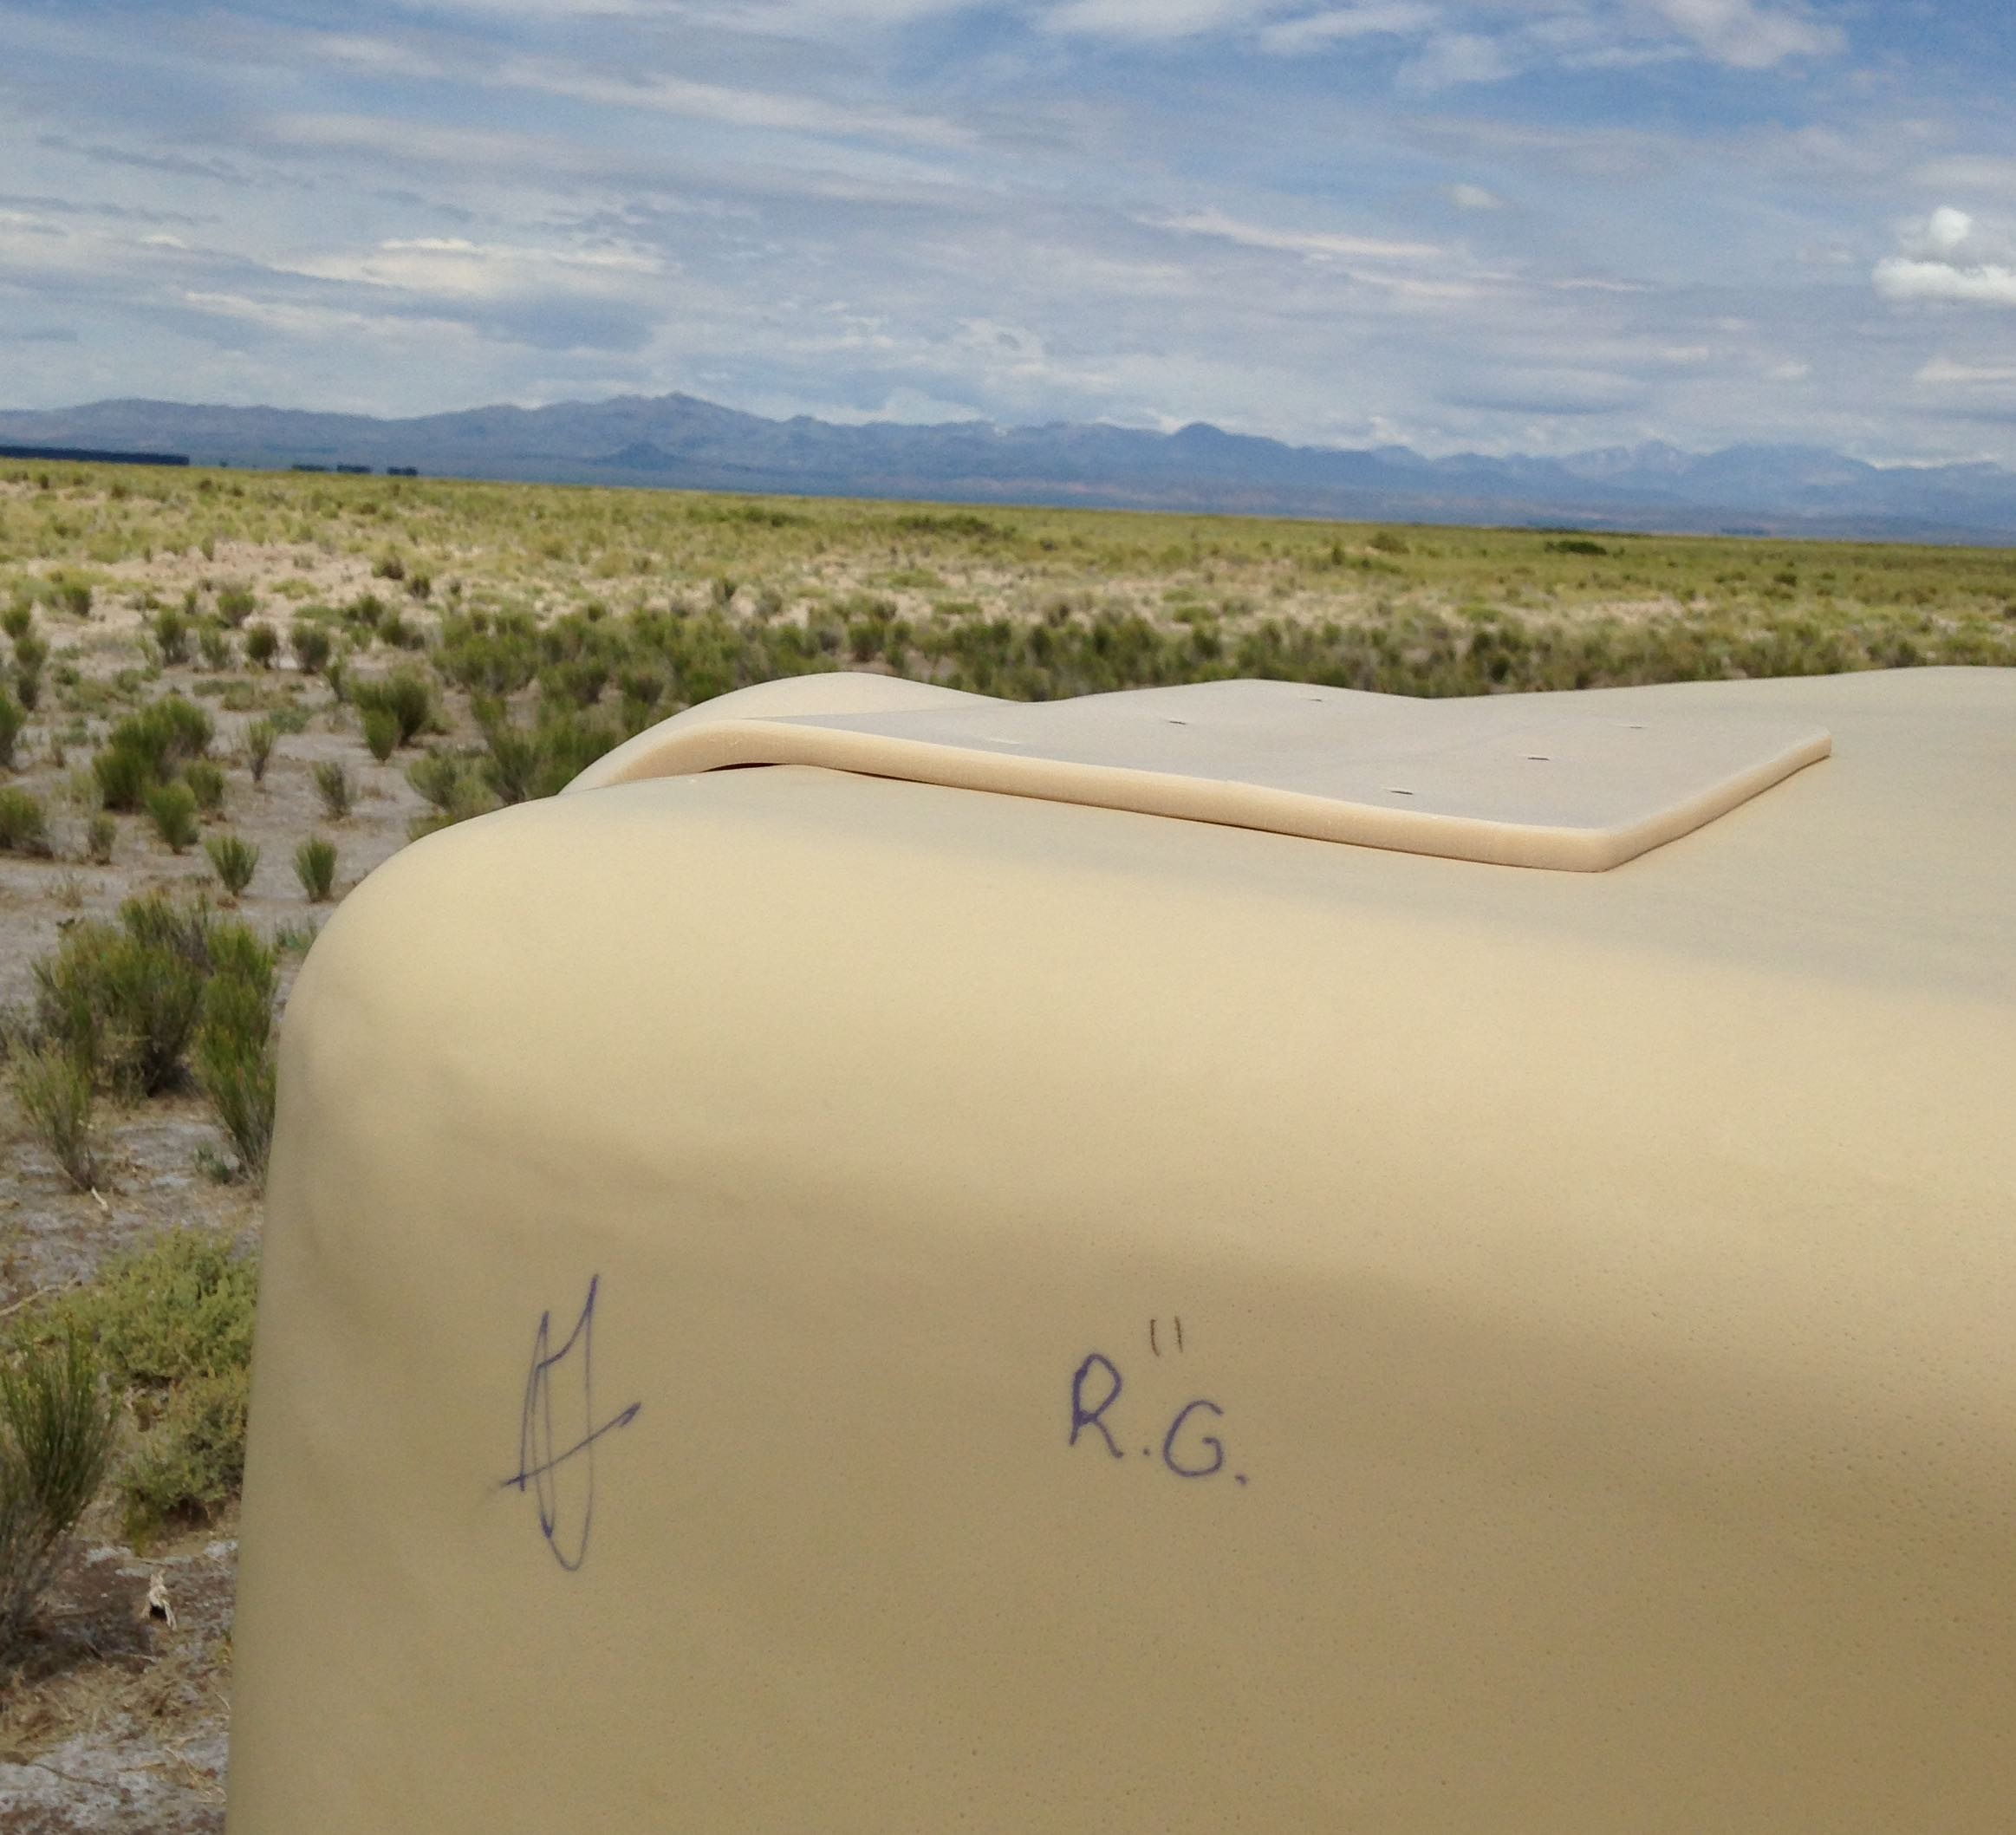
\includegraphics[width=0.49\linewidth]{signature.jpg}}
  \label{fig:monit}
\end{figure}


%%\section{Description}
lalalala

%%\include{conclusion/conclusion}

\addcontentsline{toc}{chapter}{Bibliography}                                 
\bibliographystyle{atlasnote}
\bibliography{thebib}
%% \newpage

\end{document}
